% Stanford University PhD thesis style -- modifications to the report style
% This is unofficial so you should always double check against the
% Registrar's office rules
% See http://library.stanford.edu/research/bibliography-management/latex-and-bibtex
% 
% Example of use below
% See the suthesis-2e.sty file for documentation
%
% !TEX root = main.tex
\documentclass{report}
\usepackage{suthesis-2e}
\usepackage{graphicx}
\usepackage{svg}
\usepackage{verbatim}
\usepackage{amsmath}
\usepackage{float}
\usepackage{amssymb}
\let\oldemptyset\emptyset
\let\emptyset\varnothing
% \usepackage{booktabs}
\usepackage{booktabs,float,siunitx}
% \usepackage[demo]{graphicx} % omit 'demo' option in real document
% for block comment
\usepackage{color}   % May be necessary if you want to color links
\usepackage{hyperref}
\usepackage{textcomp}
\usepackage{xcolor}
\usepackage[linesnumbered,ruled,vlined]{algorithm2e}
\usepackage{dblfloatfix}
\usepackage[backend=bibtex,style=ieee,natbib=true]{biblatex} % Use the bibtex backend with the authoryear citation style (which resembles APA)
\usepackage{listings}\definecolor{listinggray}{gray}{0.9}
\newcommand\mycommfont[1]{\footnotesize\ttfamily\textcolor{blue}{#1}}
\SetCommentSty{mycommfont}
\definecolor{lbcolor}{rgb}{0.9,0.9,0.9}
\lstset{
backgroundcolor=\color{lbcolor},
tabsize=4,
%   rulecolor=,
language=[GNU]C++,
basicstyle=\scriptsize,
upquote=true,
aboveskip={1.5\baselineskip},
columns=fixed,
showstringspaces=false,
extendedchars=false,
breaklines=true,
prebreak = \raisebox{0ex}[0ex][0ex]{\ensuremath{\hookleftarrow}},
frame=single,
numbers=left,
showtabs=false,
showspaces=false,
showstringspaces=false,
identifierstyle=\ttfamily,
keywordstyle=\color[rgb]{0,0,1},
commentstyle=\color[rgb]{0.026,0.112,0.095},
stringstyle=\color[rgb]{0.627,0.126,0.941},
numberstyle=\color[rgb]{0.205, 0.142, 0.73},
%        \lstdefinestyle{C++}{language=C++,style=numbers}’.
}
\lstset{
backgroundcolor=\color{lbcolor},
tabsize=4,
language=C++,
captionpos=b,
tabsize=3,
frame=lines,
numbers=left,
numberstyle=\tiny,
numbersep=5pt,
breaklines=true,
showstringspaces=false,
basicstyle=\footnotesize,
%  identifierstyle=\color{magenta},
keywordstyle=\color[rgb]{0,0,1},
commentstyle=\color{Darkgreen},
stringstyle=\color{red}
}

%\usepackage{xcolor}
%\lstset { %
%    numbers=left,
%    numberstyle=\tiny,
%    stepnumber=1,
%    numbersep=5pt
%    language=C++,
%%    backgroundcolor=\color{black!5}, % set backgroundcolor
%%    basicstyle=\footnotesize,% basic font setting
%}

\addbibresource{../src/mybib.bib} % The filename of the bibliography
\hypersetup{
colorlinks=false, %set true if you want colored links
linktoc=all,     %set to all if you want both sections and subsections linked
linkcolor=black,  %choose some color if you want links to stand out
}
\dept{Electronic and Information Engineering}

\begin{document}
    \title{Fast Depth Coding in 3D-HEVC
    Using Deep Learning}
    \author{Zhen-xiang WANG}
    \principaladviser{Yui-Lam Chan}
    \beforepreface
    \prefacesection{Abstract}
    The 3D Extension of the High Efficiency Video Coding standard (3D-HEVC),
    which has been finalized by the Joint Collaborative Team on Video Coding
    (JCT-VC) in February 2015, is the new industry standard for 3D applications.
    The 3D-HEVC provides plenty of advanced coding tools specifically
    for addressing the coding of auto-stereoscopic videos which have the format
    of multiple texture views along with the depth maps which are responsible
    for synthesising intermediate views with sufficient quality for
    auto-stereoscopic display.
    The provided tools take advantage of the statistical redundancies amongst
    texture views and depth maps in the video sequences, as well as the unique
    characteristics of depth maps to significantly shrink the bit-rate
    while preserving the objective visual quality of the
    3D videos.
    However, those tools with high capability in terms of compression come
    with the high complexity of computation which has made the encoding time
    of the 3D video sequences much longer than ever by traversing a lot more
    candidates, calculating time-consuming RD Cost for each of them,
    especially in the wedgelet searching process for depth maps.
    While this full-search style method can promise to find the best
    candidate in depth intra mode decision, the time cost is expensive.

    In this dissertation we address the time cost by presenting a new
    intra mode decision method for depth maps, leveraging the deep
    convolutional neural networks to predict the wedgelet angles
    for the depth blocks.
    The predictions from the learned models are capable of
    reducing the number of wedgelet candidates by half as well as the
    angular modes in depth map coding.
    The size of the neural network has been carefully designed to balance
    the trade-off between the time cost of model prediction and the model prediction
    accuracy.
    Confusion matrix is used to monitor the training process.
    Top-K criteria is employed for the prediction.
    We have integrated the learned models into the reference software of
    3D-HEVC for the experiments.
    The compiled executable binaries are able to harness
    the power of the simultaneous computation of CPU, as well as
    the parrallel computation of GPU to accelerate the predictions.
    The simulation results show that the proposed algorithm
    provides 64.6\% time reduction in average while the
    BD performance has a tiny decrease comparing with the state-of-the-art 3D-HEVC
    standard.

    \prefacesection{Acknowledgments}
%    I would not be able to accomplish the work in this dissertation
%    if it were not for the help
%    from people.
    First and foremost, I would like to give sincere thanks to my supervisor,
    Dr.Yui-Lam Chan, for his
    extremely generous support, most insightful advices and innumerable yet
    constructive feedback.
    I learned from him to first identify a problem,
    by reading a vast amount of articles
    to know what people have achieved and what bottlenecks they have encountered.
    I learned how to read papers, how to organize them to
    become the inner comprehension.
    He guided me to use the machine learning approach to solve the
    problem that has been found in the first stage.
    Without his guidance I will not have the idea to learn the deep
    learning technology and apply it to optimize the video coding.
    His encyclopedic knowledge and charming personalities made him my mentor in
    both research and life.
    I wish to thank Dr.Sik-Ho Tsang, for our in-depth discussions from
    which I can always find useful clues to proceed to next step.
    His great expertise in video coding significantly benefits me during my
    intensive period of learning.
    Also I would like to thank my friends Alex
    and Jacky, for our
    extensive discussions about artificial intelligence
    and their applications.
    Finally thank you my parents, for the great love and constant
    encouragement which give me confidence to face and handle all the
    challenges at every moment.
    \afterpreface
    \chapter{Introduction}\label{ch:chapter1} % For referencing the chapter elsewhere, use \ref{Chapter1}

%----------------------------------------------------------------------------------------
Video is the medium to record, copy, playback, broadcast
and display the motion images in an electronic style~\parencite{RN190}.
Watching videos is becoming an important way for our entertainment as well
as education.
The high definition (HD) and ultra high definition (UHD) video
are increasingly demanding nowadays.
People prefer videos with higher definitions than those with lower
resolutions because the former one provides much better viewing experience.
However, challenges emerged for delivering videos with high definition.
HD videos typically contain much more information in every picture frame than the
standard definition videos.
More data needs to be squeezed into the same capacity for transmission.
For example, the uncompressed video with the dimension 720 x 480 at 30 frames
per second requires 0.03 gigabytes per second, while the uncompressed video with
the dimension 2880 x 2048 at 120 frames per second requires 2.12 gigabytes per
second.
Since bit rate is proportional to system bandwidth for
transmission~\parencite{RN191}, and expanding the bandwidth in a large scale is
too expensive, the significantly increased bit rate
for transmitting the video data is becoming one of the
major obstacles for HD video services.\\
\newline
To cope with the growing need for higher compression of moving
pictures~\parencite{RN193}, Joint Collaborative Team on Video
Coding (JCT-VC)~\parencite{RN192} has developed the High Efficiency Video
Coding standard which is the newest international video coding standard for
substantially ameliorate the compression performance against the previous
standards.
Comparing with the H.264 Advanced Video Compression Standard~\parencite{RN194},
the H.265 High Efficiency Video Coding Standard provides fifty percent bit rate
reduction while maintaining the objective video quality at the same level.\\
\newline
While Two-dimensional video is the most common video type,
Three-dimensional (3D) video has been brought to market via lots of ways,
including Blu-Ray disc, cable and satellite transmission, terrestrial
broadcast, and streaming or downloading from the Internet~\parencite{RN118}.
3D video provides the perception of depth information which augments
the vividness of the video contents.
Currently most 3D videos in the market are using stereo display technology.
Two similar views, one for left eye, the other for right eye, are presented
at the same time with the multiplexing techniques enabling the
adjustments of video geometry information~\parencite{RN196} to provide
the 3D effect.
Figure~\ref{fig:stereo-display} illustrates the typical system structure for
transmitting videos targeting stereo display.
It can be observed that there exists a displacement between the
two views.
The green vertical left margins of the red rectangles in the two views
at encoder side are different.
Such a displacement is the visual disparity for 3D perception.
Stereoscopic videos~\parencite{RN153} have
achieved great profitability for movie theatres in recent years.
For example, IMAX 3D has became the most popular one that offering
the immersing multimedia experiences around the world.
Special 3D glasses are needed for watching the IMAX 3D movies.
The current 3D film industry is very successful in terms of attracting
customers, however, it is not the end of the story.
Myopic people do not like to wear one more pair of glasses when
watching 3D movies.
Some people will experience discomfort after wearing the 3D glasses for a
period of two hours.
Autostereoscopic multi-view technology~\parencite{RN153} is coming to our rescue.
No glasses are needed if Autostereoscopic videos can
substitute the Stereoscopic videos.
The Autostereoscopic multi-view display demands more than two
views for audience to view the 3D contents
without extra eye glasses.
The visual quality of
the Autostereoscopic display is highly correlated to the number of views
that can be provided in the receiver side.
Due to limited available bandwidth, transmitting arbitrary number of views
is not practical.
Researchers have proposed a new format which is making use of limited number
of view and their associated depth maps~\parencite{RN44}.
The typical system structure for using this new format to compress and supply 3D video
resources is shown in figure~\ref{fig:SS-MVD}.
\begin{figure}
    \centering
    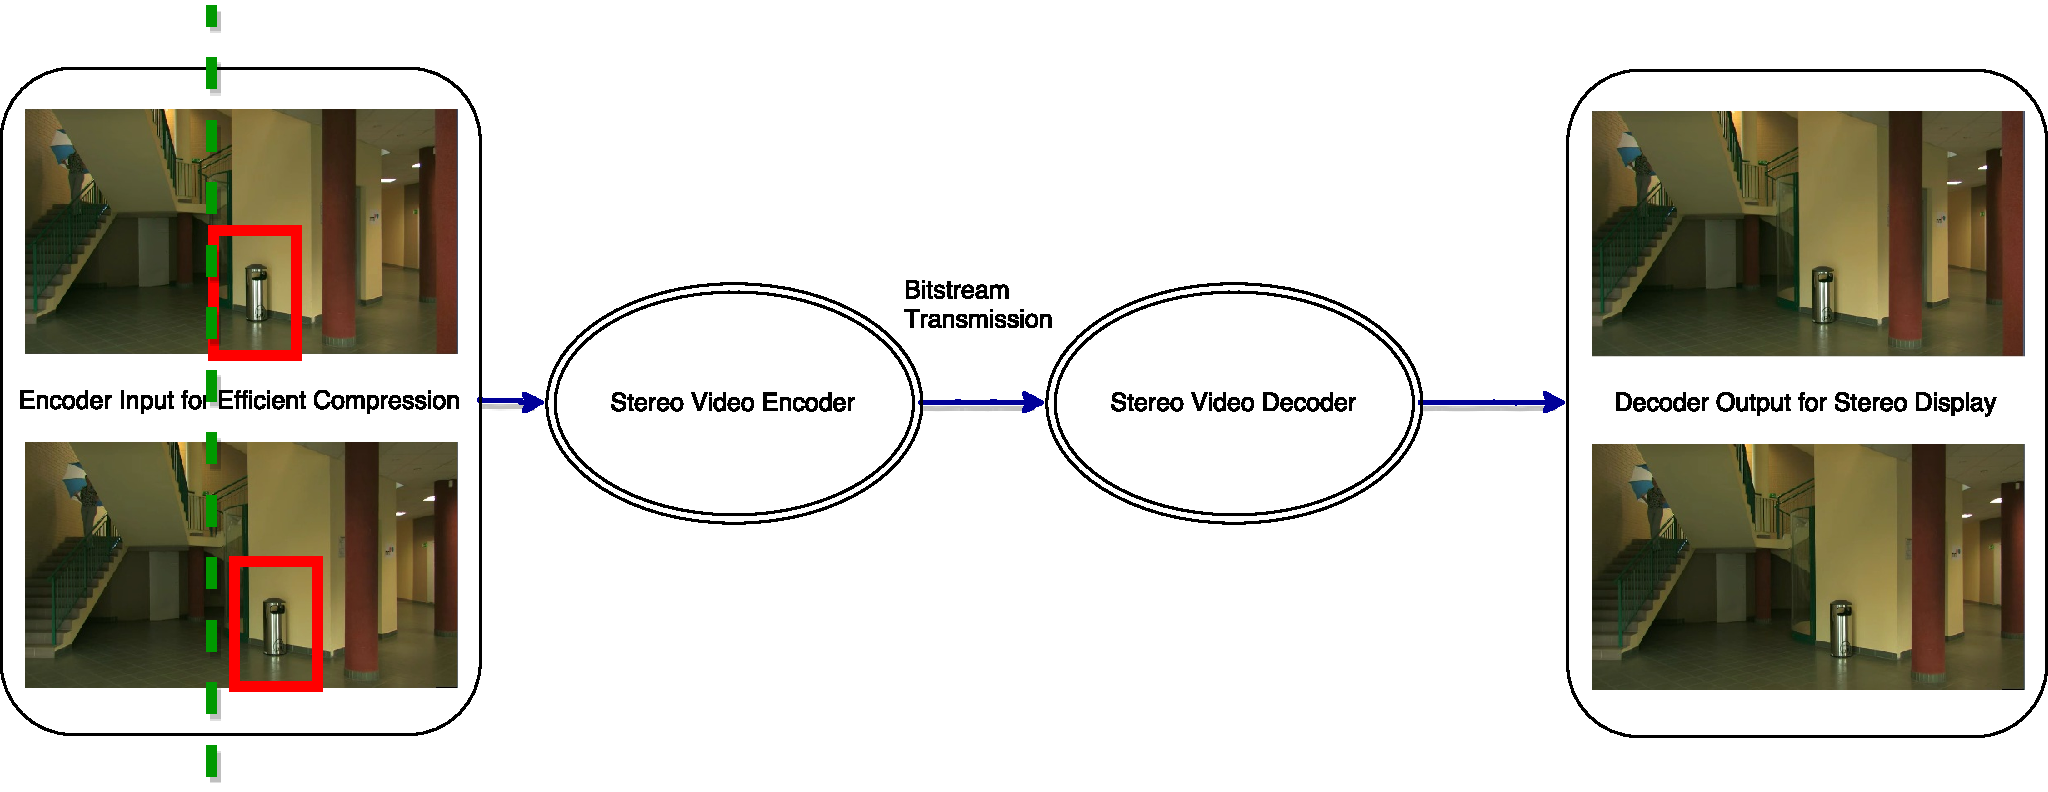
\includegraphics[width=\textwidth,height=\textheight,keepaspectratio]{Figures/StereoDisplay}
%        \decoRule
    \caption[System Structure for transmitting videos targeting stereo display]{System Structure for transmitting videos targeting stereo display.}
    \label{fig:stereo-display}
\end{figure}
An enormous amount of views in the medium positions which are able to
guarantee the high quality of the 3D video can be synthesized from
\begin{figure}
    \centering
    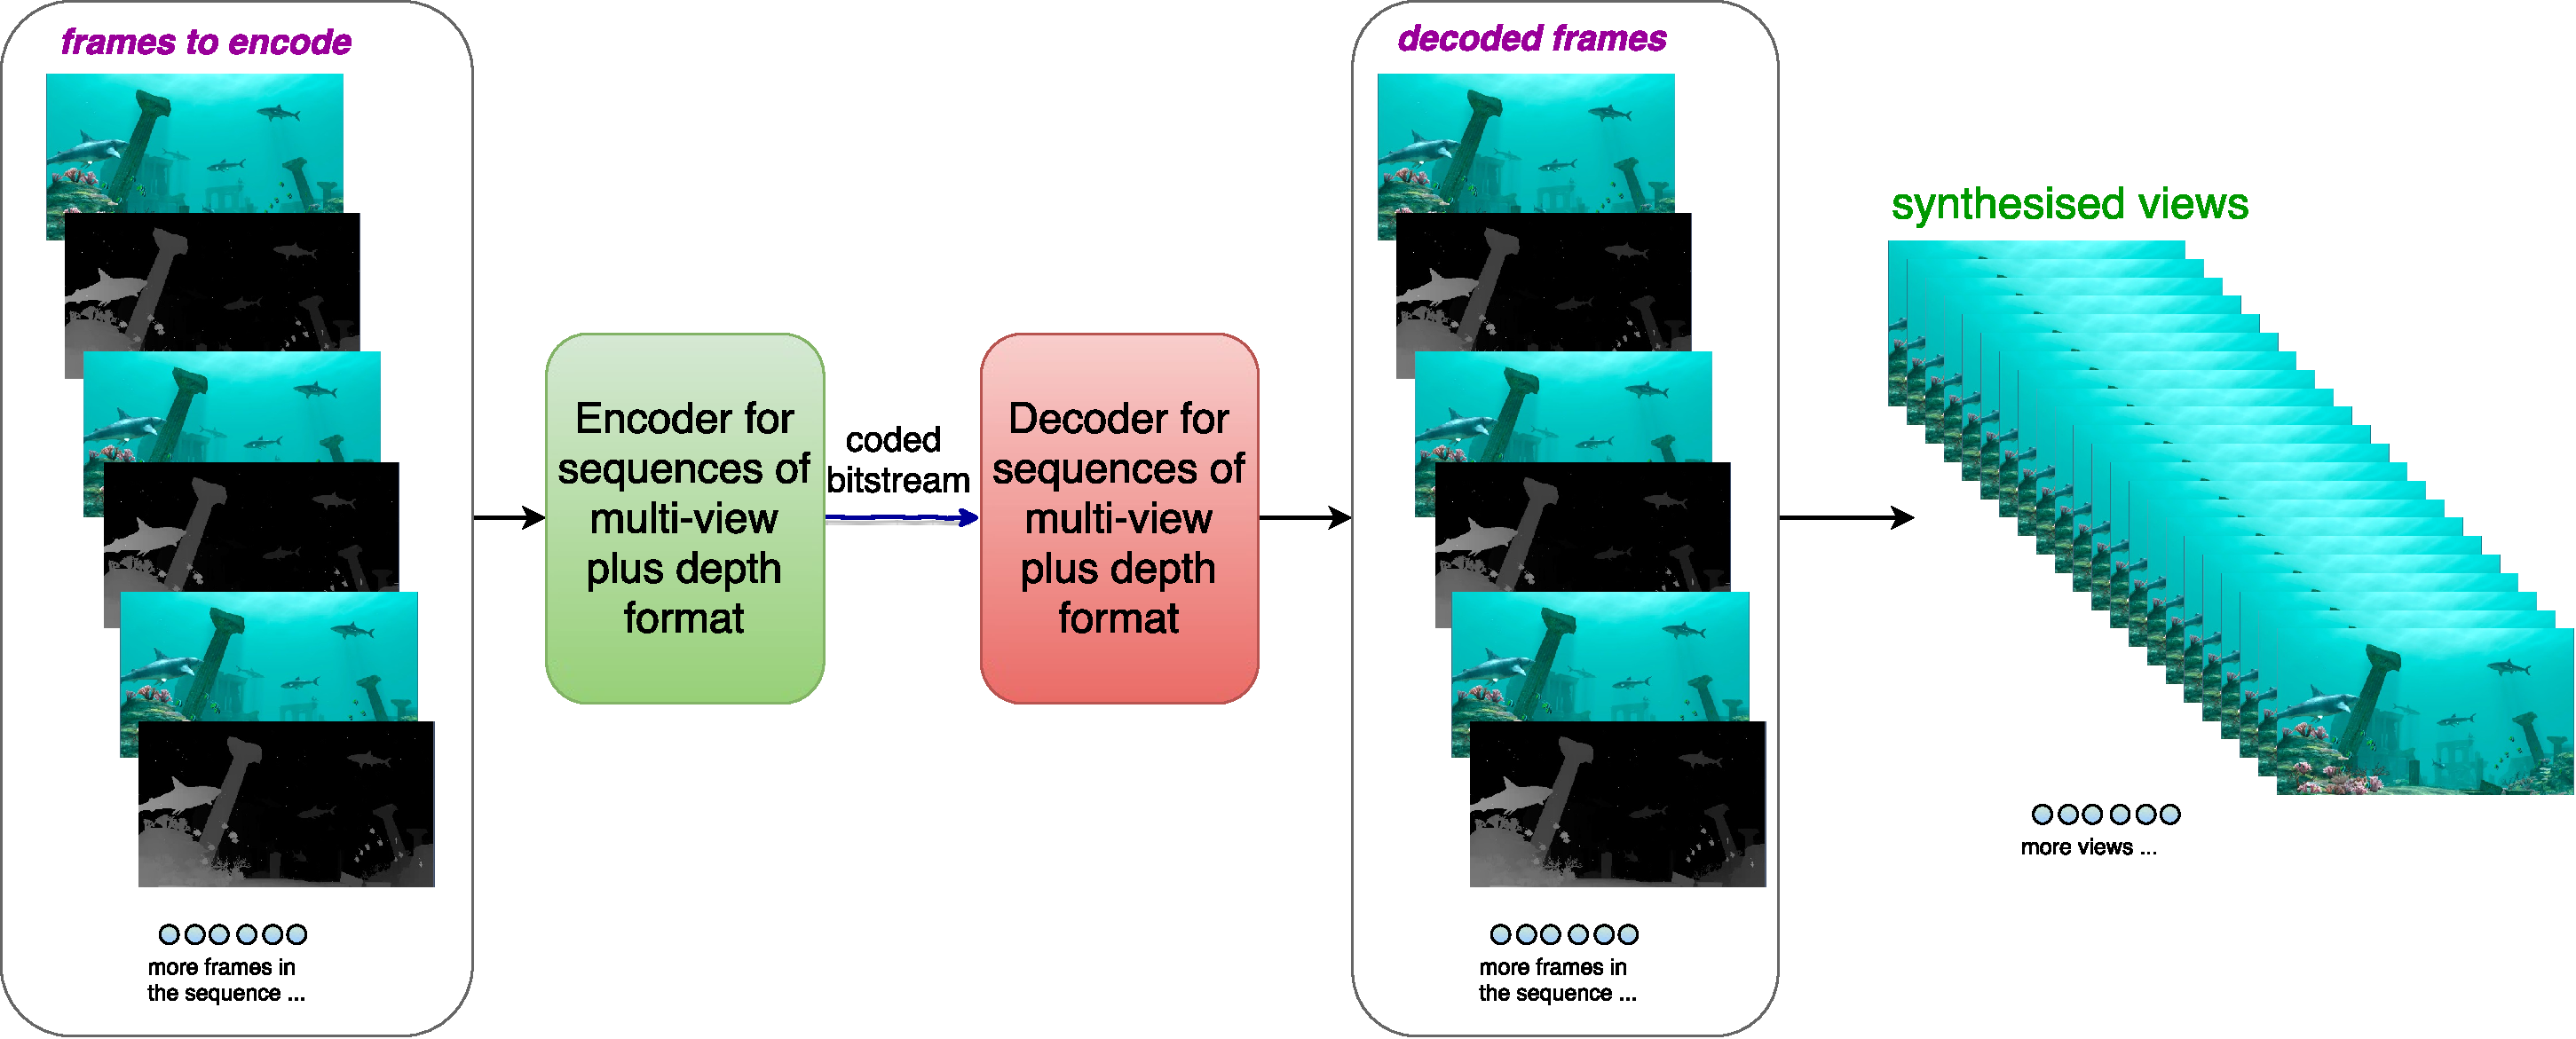
\includegraphics[width=\textwidth,height=\textheight,keepaspectratio]{Figures/SystemStructureOf3DEncoder}
%        \decoRule
    \caption[System Structure for transmitting videos of Multi-view Plus Depth format]{System Structure for transmitting videos of Multi-view Plus Depth format.}
    \label{fig:SS-MVD}
\end{figure}
the decoded texture frames in combination with decoded depth maps.\\
%The multi-view plus depth format provides the functionality of synthesizing
%required number of views from texture views and associated depth maps.\\
\newline
To employ multi-view plus depth format for 3D video, efficient compressing
methods are desired, which has led to the 3D Video Coding Extension of the
High Efficiency Video Coding Standard (3D-HEVC) by the Joint Collaborative Team
on 3D Video Coding Extension Development (JCT-3V)~\parencite{RN195}.
The 3D Extension of the HEVC standard gives extra coding efficiency
for encoding a few texture views along with the corresponding depth maps by
using new tools which exploit the redundancies amongst
texture and depth views, and pay attention to the unique characteristics of
the depth maps, such as large homogeneous
regions separated by sharp boundaries~\parencite{RN47}.\\
\newline
Depth information measures of the distance between the object in the far position
and the object in the near position from a static viewpoint,
which is expressed in the format of depth map.
Instead of presenting depth maps directly to the viewer, views in the medium
positions are generated by Depth-Image-Based Rendering (DIBR) technique.
The qualities of the depth maps are vital to the DIBR process.
Corona artifacts (a.k.a. ringing artifacts) can be discovered in synthesized
views if the edge sharpness in depth maps can not be well
preserved.
Therefore, retaining the edge sharpness in depth map is the key to avoid the
artifacts in the synthesized views.
In 3D-HEVC, new intra-picture prediction and residual coding methods
have been applied to preserve the special properties of depth
map.
Depth Modelling Mode (DMM), which is one of the new intra-picture
prediction tools, is designed to provide much more granularity for
encoding the depth maps.
Wedgelet partition and contour partition for depth maps
are enabled by DMM1 and DMM4 separately.
%~\parencite{RN197}.

%introduce a little about depth map and their usage.
%mentioning iphonex true depth camera.
%draw the picture

%----------------------------------------------------------------------------------------

\section{Motivation and Contribution}\label{sec:motivation_and_contribution}
%fasdfasdfasdfasdfasdfasdf figure~\ref{fig:SS-MVD}
If you are
\begin{table}
    \label{tab:treatments}
    \centering
    \begin{tabular}{c r @{.} l}
        Pi expression       &
        \multicolumn{2}{c}{Value} \\
        \hline
        $\pi$               & 3&1416  \\
        $\pi^{\pi}$         & 36&46   \\
        $(\pi^{\pi})^{\pi}$ & 80662&7 \\
    \end{tabular}
    \caption{The effects of treatments X and Y on the four groups studied.}
\end{table}

\begin{table}
    \label{tab:tabular_example1}
    \centering
    \begin{tabular}[t]{|r|l|}
        \hline
        7C0 & hexadecimal \\
        3700 & octal \\
        \cline{2-2} 11111000000 & binary \\
        \hline
        \hline
        1984 & decimal \\
        \hline
    \end{tabular}
\caption{Just an example}
\end{table}

\begin{table}
    \label{tab:tabular_example2}
    \centering
    \begin{tabular}{|r|l|}
        \hline
        7C0 & hexadecimal \\
        3700 & octal \\
%        \cline{2-2}
%        11111000000 & binary \\
%        \hline
%        \hline
%        1984 & decimal \\
        \hline
    \end{tabular}
\caption{Basic Usage}
\end{table}

\begin{table}
    \label{tab:tabular_example3}
    \centering
    \begin{tabular}{|r|l|}
        \hline
        7C0 & hexadecimal \\
        \cline{1-2}
        3700 & octal \\
        \cline{2-2}
        11111000000 & binary \\
        \cline{1-2}
        11111000 & binary \\
%        \hline
%        \hline
%        1984 & decimal \\
        \hline
    \end{tabular}
\caption{horizontal lines extend over multiple columns}
\end{table}

\begin{table}
    \label{tab:tabular_example4}
    \centering
    \begin{tabular}{|p{4.7cm}|}
        \hline Welcome to Boxy's paragraph. We sincerely hope you'll all enjoy the show.\\
        \hline
    \end{tabular}
    \caption{define a special type of column which will wrap-around the text as in a normal paragraph}
\end{table}

\begin{table}
    \label{tab:tabular_example8}
    \centering
    \begin{tabular}{p{4.7cm}}
        \hline
        Welcome to Boxy's paragraph.
        We sincerely hope you'll all enjoy the show.\\
        \hline
    \end{tabular}
    \caption{define a special type of column which will wrap-around the text as in a normal paragraph}
\end{table}

\begin{table}
    \label{tab:tabular_example5}
    \centering
    \begin{tabular}{@{} l @{}}
        \hline Welcome to Boxy's paragraph. We sincerely hope you'll all enjoy the show.\\
        \hline
    \end{tabular}
    \caption{define a special type of column which will wrap-around the text as in a normal paragraph}
\end{table}

\begin{table}
    \label{tab:tabular_example6}
    \centering
    \begin{tabular}{l}
        \hline Welcome to Boxy's paragraph. We sincerely hope you'll all enjoy the show.\\
        \hline
    \end{tabular}
    \caption{define a special type of column which will wrap-around the text as in a normal paragraph}
\end{table}

\begin{table}
    \label{tab:tabular_example9}
    \centering
    \begin{tabular}{c c} \hline \multicolumn{2}{c}{Ene} \\ \hline Mene & Muh! \\ \hline \end{tabular}
    \caption{multicolumn command}
\end{table}

\begin{table}
    \label{tab:tabular_example10}
    \centering
    \begin{tabular}{c c c c c c}
        \hline
        sequence name &
        BD-BR &
        \multicolumn{4}{c}{Ene} \\
        \cline{3-6}
        {} & {} & Me & Muh & Me & Mu\\
        \hline
        Newspaper & 0.98\% & 22 & 33 & 44 & 66\\
    \end{tabular}
    \caption{multicolumn command}
\end{table}




%\begin{table}
%    \label{tab:treatments}
%    \centering
%    \begin{tabular}{c r @{.} l}
%        Pi expression       &
%        \multicolumn{2}{c}{Value} \\
%        \hline
%        $\pi$               & 3&1416  \\
%        $\pi^{\pi}$         & 36&46   \\
%        $(\pi^{\pi})^{\pi}$ & 80662&7 \\
%    \end{tabular}
%    \caption{The effects of treatments X and Y on the four groups studied.}
%\end{table}
%----------------------------------------------------------------------------------------

\section{Dissertation Outline}\label{sec:outline}




%\chapter{Introduction}\label{ch:chapter1} % For referencing the chapter elsewhere, use \ref{Chapter1}
%
%%----------------------------------------------------------------------------------------
%
%%----------------------------------------------------------------------------------------
%
%\section{Welcome and Thank You}\label{sec:welcome}
%Welcome to this \LaTeX{} Thesis Template, a beautiful and easy to use template for writing a thesis using the \LaTeX{} typesetting system.
%
%If you are writing a thesis (or will be in the future) and its subject is technical or mathematical (though it doesn't have to be), then creating it in \LaTeX{} is highly recommended as a way to make sure you can just get down to the essential writing without having to worry over formatting or wasting time arguing with your word processor.
%
%\LaTeX{} is easily able to~\parencite{RN93} professionally typeset documents that run to hundreds or thousands of pages long. With simple mark-up commands, it automatically sets out the table of contents, margins, page headers and footers and keeps the formatting consistent and beautiful. One of its main strengths is the way it can easily typeset mathematics, even \emph{heavy} mathematics. Even if those equations are the most horribly twisted and most difficult mathematical problems that can only be solved on a super-computer, you can at least count on \LaTeX{} to make them look stunning.
%
%%----------------------------------------------------------------------------------------
%
%\section{Welcome and Thanku}\label{sec:welome}
%Welcome to this \LaTeX{} Thesis Template, a beautiful and easy to use template for writing a thesis using the \LaTeX{} typesetting system.
%
%If you are writing a thesis (or will be in the future) and its subject is technical or mathematical (though it doesn't have to be), then creating it in \LaTeX{} is highly recommended as a way to make sure you can just get down to the essential writing without having to worry over formatting or wasting time arguing with your word processor.
%
%\LaTeX{} is easily able to professionally typeset documents that run to hundreds or thousands of pages long. With simple mark-up commands, it automatically sets out the table of contents, margins, page headers and footers and keeps the formatting consistent and beautiful. One of its main strengths is the way it can easily typeset mathematics, even \emph{heavy} mathematics. Even if those equations are the most horribly twisted and most difficult mathematical problems that can only be solved on a super-computer, you can at least count on \LaTeX{} to make them look stunning.
%
%%----------------------------------------------------------------------------------------
%
%\section{Welcome and ThYou}\label{sec:weome}
%Welcome to this \LaTeX{} Thesis Template~\parencite{Reference1}, a beautiful and easy to use template for writing a thesis using the \LaTeX{} typesetting system.
%
%If you are writing a thesis (or will be in the future) and its subject is technical or mathematical (though it doesn't have to be), then creating it in \LaTeX{} is highly recommended as a way to make sure you can just get down to the essential writing without having to worry over formatting or wasting time arguing with your word processor.
%
%\LaTeX{} is easily able to professionally typeset documents that run to hundreds or thousands of pages long. With simple mark-up commands, it automatically sets out the table of contents, margins, page headers and footers and keeps the formatting consistent and beautiful. One of its main strengths is the way it can easily typeset mathematics, even \emph{heavy} mathematics. Even if those equations are the most horribly twisted and most difficult mathematical problems that can only be solved on a super-computer, you can at least count on \LaTeX{} to make them look stunning.
%
%%----------------------------------------------------------------------------------------
%
%\section{Welcome and Thau}\label{sec:welcoe}
%Welcome to this \LaTeX{} Thesis Template, a beautiful and easy to use template for writing a thesis using the \LaTeX{} typesetting system.
%
%If you are
%\begin{table}
%
%    \label{tab:treatments}
%    \centering
%%    \begin{tabular}{l l l}
%%        \toprule
%%        \tabhead{Groups} & \tabhead{Treatment X} & \tabhead{Treatment Y} \\
%%        \midrule
%%        1 & 0.2 & 0.8\\
%%        2 & 0.17 & 0.7\\
%%        3 & 0.24 & 0.75\\
%%        4 & 0.68 & 0.3\\
%%        \bottomrule\\
%%    \end{tabular}
%    \begin{tabular}{c r @{.} l}
%        Pi expression       &
%        \multicolumn{2}{c}{Value} \\
%        \hline
%        $\pi$               & 3&1416  \\
%        $\pi^{\pi}$         & 36&46   \\
%        $(\pi^{\pi})^{\pi}$ & 80662&7 \\
%    \end{tabular}
%    \caption{The effects of treatments X and Y on the four groups studied.}
%\end{table}
%writing a thesis (or will be in the future) and its subject is technical or mathematical (though it doesn't have to be), then creating it in \LaTeX{} is highly recommended as a way to make sure you can just get down to the essential writing without having to worry over formatting or wasting time arguing with your word processor.
%
%\LaTeX{} is easily able to professionally typeset documents that run to hundreds or thousands of pages long. With simple mark-up commands, it automatically sets out the table of contents, margins, page headers and footers and keeps the formatting consistent and beautiful. One of its main strengths is the way it can easily typeset mathematics, even \emph{heavy} mathematics. Even if those equations are the most horribly twisted and most difficult mathematical problems that can only be solved on a super-computer, you can at least count on \LaTeX{} to make them look stunning.
%
%%----------------------------------------------------------------------------------------
%
%\section{Welcome and Tnk You}\label{sec:wlcome}
%Welcome to this \LaTeX{} Thesis Template, a beautiful and easy to use template for writing a thesis using the \LaTeX{} typesetting system.
%
%If you are writing a thesis.
%
%%\begin{verbatim}
%\begin{figure}
%    \centering
%    
\includegraphics{Figures/Electron}
%    %    \decoRule
%    \caption[An Electron]{An electron (artist's impression).}
%    \label{fig:Electron}
%\end{figure}
%%\end{verbatim}
%(or will be in the future) and its subject is technical or mathematical (though it doesn't have to be), then creating it in \LaTeX{} is highly recommended as a way to make sure you can just get down to the essential writing without having to worry over formatting or wasting time arguing with your word processor.
%
%\LaTeX{} is easily able to professionally typeset documents that run to hundreds or thousands of pages long. With simple mark-up commands, it automatically sets out the table of contents, margins, page headers and footers and keeps the formatting consistent and beautiful. One of its main strengths is the way it can easily typeset mathematics, even \emph{heavy} mathematics. Even if those equations are the most horribly twisted and most difficult mathematical problems that can only be solved on a super-computer, you can at least count on \LaTeX{} to make them look stunning.
%
%%----------------------------------------------------------------------------------------

    \chapter{Background}\label{ch:chapter2} % For referencing the chapter elsewhere, use \ref{Chapter1}
%
%%----------------------------------------------------------------------------------------
%
To start with, we bring up what is video coding, why it is needed, and
its challenges.
Next we discuss what is deep learning, the history of deep learning and how
it works for vision tasks.
Furthermore, we introduce how we plan to apply deep learning to optimize video
coding tasks and why it should work.
In the end, a survey of related works in video coding and deep learning is given.

%3D Video applications are attracting more interests
%%----------------------------------------------------------------------------------------
%
\section{Video Coding}\label{sec:video-coding}
Video playback is the most straightforward way for human to perceive dynamic
scenes that exist across a time series.
More than half of the neurons in human brain are born to process the visual
information which is supplied by human eyes.
It becomes effortless for human to understand things presented by
the video playback instead of a long paragraph of words.
Videos are made up of consecutive sets of image frames, which in turn
are made up of pixel matrices.
Visual information of a cosmic scale is first stored by various methods
then delivered during a period of video playback.

In 1950s, video tapes were employed to store the videos.
Video tape is able to serve for about eight to twelve years
before the video quality starts to degrade.
In 1970s, laser disc appeared in the US market as an alternative of video tapes.
Start from laser disc, the video storage started its new era in digital world.
In 1990s, DVDs were released after laser disc.
Data is stored in spiralling tracks on the disc.
A laser beam can be utilized to read the data.
In addition, hard drives, flash drives and SD cards were also starting to
become popular in the late 90s.
Nowadays, the cloud storage is very common in daily lives.
It is capable of storing data on the servers which are
accessible from any devices via internet connections.

Although so many formats are available for video storage, they share a common
feature: the more storage you use, the more cost it will be.
Let's take the cloud storage as an example.
Google cloud is one of the most popular cloud services in our daily lives.
It provides cloud storage with a price
of \$0.026 per GB/month~\parencite{RN202}
(this price is observed on 21 Nov 2017, it may change in the future).
If a 4K video with a resolution of 4096*2160,
at 120 frames per second,
8 bits for each of the RGB component, needs to be stored without
any compression in Google cloud,
we need to pay a monthly fee:
\((4096*2160*120*60*90*3*0.026)/(1024*1024*1024) \approx 416.47\) \$.
Without doubt, this figure is relatively not acceptable for just
storing the video.
High compression is needed to store the videos in a practical way.

From the other perspective, let us take the bandwidth into consideration.
To deliver the uncompressed 4K video which has been mentioned in
the previous paragraph, we need a bandwidth of:
\((4096*2160*120*3)/(1024*1024*1024) \approx 2.97\) Gigabytes per second.
The maximum bandwidth of Wireless 802.11ac, which is one of the common
internet access technologies, is 1.3 Gigabytes per second~\parencite{RN203}.
Apparently, the wireless connection is not able to deliver such kind of
4K videos.
High compression is desired to deliver the video through the internet.

Despite the fact that raw videos usually contain a large amount of data,
a lot of redundancies exist.
For every video sequence, two types of redundancies are ubiquitous: Spacial
Redundancy and Temporal Redundancy.
Video coding technologies are taking advantages of those redundancies to
achieve the efficient compression for video data.
Many of the useful video coding technologies have been adopted by the
international video coding standards, such as MPEG-4, H.264, H.265, etc.

Figure~\ref{fig:video-std-brief-history} shows the brief history of the
video coding standards.
\begin{figure}
    \centering
    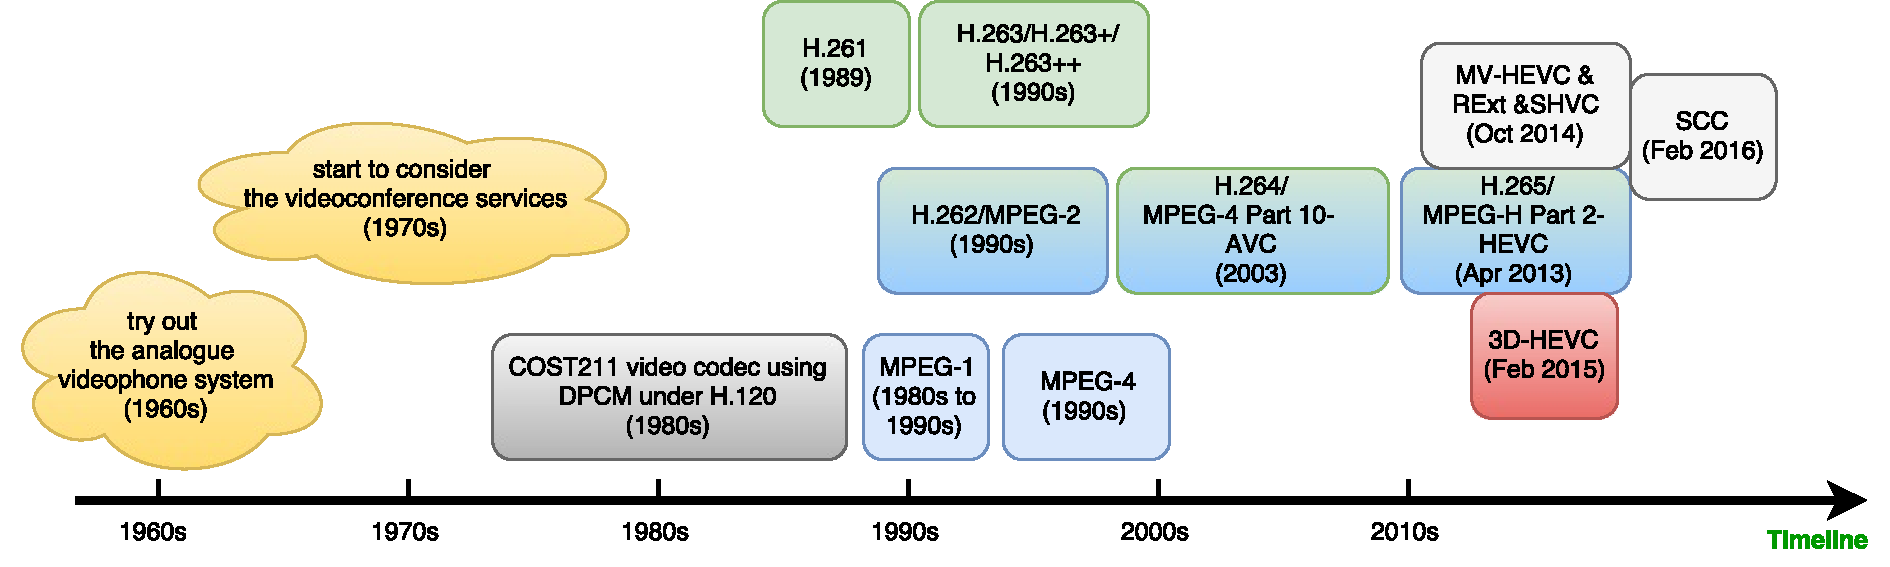
\includegraphics[width=\textwidth,height=\textheight,keepaspectratio]{Figures/video-std-brief-history.pdf}
%        \decoRule
    \caption[The brief history of the video coding standards]
    {The brief history of the video coding standards}
    \label{fig:video-std-brief-history}
\end{figure}
In 1980s, the COST211 video codec, built on top of Differential
Pulse Code Modulation (DPCM), was standardized under H.120 standard by CCITT
(now known as ITU-T).
In late 1989, the H.261 was completed and its success marked a milestone for
video coding at low bit rate with fairly good quality~\parencite{RN181}.
The Motion Picture Experts Group (MPEG) kicked off the exploration of video
storage, such as CD-ROMs.
Their objective was to achieve a competitive performance with cassette
recorders in terms of compression of videos which have rich motions.
The framework of H.261 had been used to start the codec design of MPEG-1.
MPEG-2 was one generation after the MPEG-1.
It featured higher capabilities when handling videos with
high bit rates and high resolutions.
In MPEG-2, the encoder is allowed to make its own decision on the
the number of bi-directionally predicted pictures according to a
suitable coding delay.
ITU-T found this technique applicable to telecommunication applications, as
a result MPEG-2 has been adopted as H.262 for telecommunications.
Right after the MPEG-2 standard, MPEG-3 was designed mainly for coding of
high definition videos.
However, MPEG-3 was discarded due to the versatility of MPEG-2, which
can be used to encode videos of any resolutions.
In the late 1998, MPEG-4 was introduced as a way of defining compression of
both audio and visual digital data.
Later on MPEG-4 was divided into several parts during its continuously evolving.
Among its sub-parts, MPEG-4 part 10 (a.k.a. Advanced Video Coding) is mainly
for the video compression.
With the rising popularity of the high definition videos, the new standard
termed High Efficiency Video Coding (HEVC) for compressing videos in a more
efficient way comparing with previous standards, such as H.264/AVC, has
emerged under the efforts from the Joint Collaborative Team on Video
Coding (JCT-VC).
In the meanwhile, five extensions of the HEVC standard, comprising
Format Range Extension (RExt), Scalability Extension (SHVC),
Multi-view Extension (MV-HEVC), 3D Extension (3D-HEVC),
Screen Content Coding Extension (SCC),  have been finalized
from 2014 to 2016 to fulfill extra requirements in various video coding
scenarios.

In this work, we focus on the depth map coding in 3D-HEVC\@.
The 35 angular modes and depth modeling modes have been embraced in the
depth map coding tools in 3D-HEVC\@.
The DMM1 mode introduces an huge increase for the encoding time of 3D videos.
Acceleration of the depth map coding is needed.

\section{Deep Learning}\label{sec:deep-learning}
Deep learning is an approach of representation learning
(a.k.a. feature learning), which is essentially a method to
learn from data.
Numerous layers of computational units together with appropriate activating
mechanism comprise the basic architecture for deep learning.
Multitudinous data sets are needed for those computational architectures
to learn data abstractions for tasks such as image classification,
speech recognition, object detection, etc.
Each layer learns a level of abstraction from the data sets using
back-propagation algorithm~\parencite{RN204}.
Making use of those learned abstractions, the computational architectures are
able to solve complex problems which are typically non-linear and normally hard
to solve by using specific rules that are designed in advance.

Deep learning has been attracting wide attention from all over the world
in recent years, not only because of the great achievements it has
made in various application scenarios, but also due to the promise of an
intelligent future it gives.
Such a learning methodology makes people believe it is possible
for the formation of wise machines
that they have long dreamed to possess.
The growing data accessibility provides rich examples for deep computational
architectures to adjust their internal weights and bias until their
predictions have low error rate.
On the other hand, the computational devices are relatively
affordable than in the previous years by the society, with the help of which,
accelerations of learning processes has been achieved, hence a bunch of
time consuming deep learning architectures can be tried within acceptable
periods.

In the ILSVRC-2012 competition~\parencite{RN205}, AlexNet~\parencite{RN65}
received the championship with the 15.3\% top-5 error rate, compared to
26.2\% achieved by the runner-up.
Such a large margin of error rate claimed a breakthrough in
object recognition history.
It kicked off a blistering pace of trying out deep learning by both academia
and industry, which in turn led to an increase of the convolutional
neural networks' submissions to ILSVRC-2013, in which ZF Net~\parencite{RN66}
was the winner.
It fine-turned the architecture of AlexNet based on the
gorgeous visualizations of trained models.
Both AlexNet and ZF Net are of the same structure which is built up
by simply stacking computational layers while GoogLeNet~\parencite{RN60}
is composed of Inception
modules.
This new architecture was the most successful candidate in ILSVRC-2014.
It has not only set the new height of object recognition but also started to
optimize the computational resources of the network by design.
It consists of 22 layers, which was deeper than all the previous
networks in ILSVRC\@.
However, it is still not deep enough.
In the ILSVRC-2015, Residual Neural Network (ResNet)~\parencite{RN67} with
152 layers won the championships in all the five main tracks.
ResNet introduced a brand new notion into the neural network architecture
named identity mapping.
The shortcut connection in the identity mapping prevents the degradation of
training accuracy when the network goes deeper.
Besides, the converging speed of ResNet is faster than the network built up
with Inception modules when both are of the similar size.

Despite the fact that neural networks built up from Inception modules
converges slower than those built up from ResNet modules, it is still
worth it for a brief review of the valuable insights residing in
the Inception networks.
A typical incarnation of the first generation of Inception networks is named
GoogLeNet~\parencite{RN60}.
It was intricately carved with a responsibility to win computer vision
tasks in ILSVRC-2014, on which it performed better than all the other
deep neural network architectures.
There exist philosophical reflections which are intend to serve as guidelines
for the construction of Inception networks.
Two major downsides of a enlarged neural network have been discussed
in~\parencite{RN60}.
One is the higher chances of overfitting while the other is
the strikingly increased requirements of computational resources with the
enlarged network size.
For handling those drawbacks, based on the new ideas which were introduced
in~\parencite{RN207} about how to construct the reasonable architecture of
neural networks, new experiments orienting sparse network structure have
been tried out.
One year later after GoogleNet stolen the show in 2014,



% ====== can be used for literature review =====
%AlexNet contains five convolutional layers and three fully-connected
%layers.
%The Rectified Linear Units (ReLU)~\parencite{RN206}, Local Response
%Normalization and Overlapping Pooling were adopted.
%The methodology of multiple GPU training was used to make the learning fast.
%Data Augmentation and Dropout were chosen to overcome the problem of
%Overfitting.
%Stochastic gradient descent was adopted.
% ====== can be used for literature review =====




%Welcome to this \LaTeX{} Thesis Template, a beautiful and easy to use template for writing a thesis using the \LaTeX{} typesetting system.
%
%If you are writing a thesis (or will be in the future) and its subject is technical or mathematical (though it doesn't have to be), then creating it in \LaTeX{} is highly recommended as a way to make sure you can just get down to the essential writing without having to worry over formatting or wasting time arguing with your word processor.
%
%\LaTeX{} is easily able to~\parencite{RN93} professionally typeset documents that run to hundreds or thousands of pages long. With simple mark-up commands, it automatically sets out the table of contents, margins, page headers and footers and keeps the formatting consistent and beautiful. One of its main strengths is the way it can easily typeset mathematics, even \emph{heavy} mathematics. Even if those equations are the most horribly twisted and most difficult mathematical problems that can only be solved on a super-computer, you can at least count on \LaTeX{} to make them look stunning.
%
%%----------------------------------------------------------------------------------------
%
%\section{Welcome and Thanku}\label{sec:welome}
%Welcome to this \LaTeX{} Thesis Template, a beautiful and easy to use template for writing a thesis using the \LaTeX{} typesetting system.
%
%If you are writing a thesis (or will be in the future) and its subject is technical or mathematical (though it doesn't have to be), then creating it in \LaTeX{} is highly recommended as a way to make sure you can just get down to the essential writing without having to worry over formatting or wasting time arguing with your word processor.
%
%\LaTeX{} is easily able to professionally typeset documents that run to hundreds or thousands of pages long. With simple mark-up commands, it automatically sets out the table of contents, margins, page headers and footers and keeps the formatting consistent and beautiful. One of its main strengths is the way it can easily typeset mathematics, even \emph{heavy} mathematics. Even if those equations are the most horribly twisted and most difficult mathematical problems that can only be solved on a super-computer, you can at least count on \LaTeX{} to make them look stunning.
%
%%----------------------------------------------------------------------------------------
%
%\section{Welcome and ThYou}\label{sec:weome}
%Welcome to this \LaTeX{} Thesis Template~\parencite{Reference1}, a beautiful and easy to use template for writing a thesis using the \LaTeX{} typesetting system.
%
%If you are writing a thesis (or will be in the future) and its subject is technical or mathematical (though it doesn't have to be), then creating it in \LaTeX{} is highly recommended as a way to make sure you can just get down to the essential writing without having to worry over formatting or wasting time arguing with your word processor.
%
%\LaTeX{} is easily able to professionally typeset documents that run to hundreds or thousands of pages long. With simple mark-up commands, it automatically sets out the table of contents, margins, page headers and footers and keeps the formatting consistent and beautiful. One of its main strengths is the way it can easily typeset mathematics, even \emph{heavy} mathematics. Even if those equations are the most horribly twisted and most difficult mathematical problems that can only be solved on a super-computer, you can at least count on \LaTeX{} to make them look stunning.
%
%%----------------------------------------------------------------------------------------
%
%\section{Welcome and Thau}\label{sec:welcoe}
%Welcome to this \LaTeX{} Thesis Template, a beautiful and easy to use template for writing a thesis using the \LaTeX{} typesetting system.
%
%If you are
%\begin{table}
%
%    \label{tab:treatments}
%    \centering
%%    \begin{tabular}{l l l}
%%        \toprule
%%        \tabhead{Groups} & \tabhead{Treatment X} & \tabhead{Treatment Y} \\
%%        \midrule
%%        1 & 0.2 & 0.8\\
%%        2 & 0.17 & 0.7\\
%%        3 & 0.24 & 0.75\\
%%        4 & 0.68 & 0.3\\
%%        \bottomrule\\
%%    \end{tabular}
%    \begin{tabular}{c r @{.} l}
%        Pi expression       &
%        \multicolumn{2}{c}{Value} \\
%        \hline
%        $\pi$               & 3&1416  \\
%        $\pi^{\pi}$         & 36&46   \\
%        $(\pi^{\pi})^{\pi}$ & 80662&7 \\
%    \end{tabular}
%    \caption{The effects of treatments X and Y on the four groups studied.}
%\end{table}
%writing a thesis (or will be in the future) and its subject is technical or mathematical (though it doesn't have to be), then creating it in \LaTeX{} is highly recommended as a way to make sure you can just get down to the essential writing without having to worry over formatting or wasting time arguing with your word processor.
%
%\LaTeX{} is easily able to professionally typeset documents that run to hundreds or thousands of pages long. With simple mark-up commands, it automatically sets out the table of contents, margins, page headers and footers and keeps the formatting consistent and beautiful. One of its main strengths is the way it can easily typeset mathematics, even \emph{heavy} mathematics. Even if those equations are the most horribly twisted and most difficult mathematical problems that can only be solved on a super-computer, you can at least count on \LaTeX{} to make them look stunning.
%
%%----------------------------------------------------------------------------------------
%
%\section{Welcome and Tnk You}\label{sec:wlcome}
%Welcome to this \LaTeX{} Thesis Template, a beautiful and easy to use template for writing a thesis using the \LaTeX{} typesetting system.
%
%If you are writing a thesis.
%
%%\begin{verbatim}
%\begin{figure}
%    \centering
%    
\includegraphics{Figures/Electron}
%    %    \decoRule
%    \caption[An Electron]{An electron (artist's impression).}
%    \label{fig:Electron}
%\end{figure}
%%\end{verbatim}
%(or will be in the future) and its subject is technical or mathematical (though it doesn't have to be), then creating it in \LaTeX{} is highly recommended as a way to make sure you can just get down to the essential writing without having to worry over formatting or wasting time arguing with your word processor.
%
%\LaTeX{} is easily able to professionally typeset documents that run to hundreds or thousands of pages long. With simple mark-up commands, it automatically sets out the table of contents, margins, page headers and footers and keeps the formatting consistent and beautiful. One of its main strengths is the way it can easily typeset mathematics, even \emph{heavy} mathematics. Even if those equations are the most horribly twisted and most difficult mathematical problems that can only be solved on a super-computer, you can at least count on \LaTeX{} to make them look stunning.
%
%%----------------------------------------------------------------------------------------
    % !TEX root = ../main.tex
\chapter{Prepare the Data for Deep Learning}\label{ch:chapter3} % For referencing the chapter elsewhere, use \ref{Chapter1}

The success of a deep learning procedure heavily relies
on the size of available data.
It only works when a considerably large set of data can be provided.
Moreover, since we are using supervised learning which is the most
popular form of deep learning for the time being, our datasets
must be well labeled.
A large dataset can contain enormous and different classes,
with each class has its own label.
The labels are used to adjust the inner parameters of a pre-constructed
deep model according to the pre-defined loss function during the training
process.
We need to prepare a large set of labeled data before starting the
model training.
In this chapter, we start with the data collection, in which the data source
and method for collecting data are shown in detail.
After that the necessary pre-processing for the collected data are described.
Furthermore, plenty of visualizations for the collected raw data are shown with
discussion explaining the reason for the data pre-processing.

\section{Data Collection}\label{sec:data-collection}
To collect the data for training a deep model to predict the most probable
intra angular directions for depth blocks, we need to identify two questions:
Firstly, where does the data come from?
Secondly, how to collect the data from the source?
In this section, the two questions are answered one by one.

\subsection{Source of Data}\label{subsec:source-of-data}
The data are collected from four video sequences as shown in
Table~\ref{tab:data-source}.
\begin{table}[t]
    \caption{Source of data for deep learning}
    \bigskip
    \label{tab:data-source}
    \centering
    \begin{tabular}{c c c c c}
        \hline
        \# & Name of the Sequence & Resolution & Usage & Number of Frames\\
        \hline
        1 & Balloons & $1024\times768$ & train,test,validate & 300\\
        2 & Kendo & $1024\times768$ & train,test,validate & 300\\
        3 & Poznan Street & $1920\times1088$ & train,test,validate & 250\\
        4 & Undo Dancer & $1920\times1088$ & train,test,validate & 250\\
        \hline
    \end{tabular}
\end{table}
Balloons sequence and Kendo sequence are of the resolution 1024 by 768 while
Poznan Street sequence and Undo Dancer sequence are of the resolution 1920
by 1088.
Both of the former two sequences have 300 frames, all of which are used to
collect the data.
The latter two sequences both have 250 frames, and all the frames are involved
in the data collection.
The collected data for each sequence will be separated into three sets
for training, testing and validating.
The training data sets are used for the deep model to learn the best
representations by the back-propagation algorithm~\parencite{RN204},
during which the inner parameters typically weights and bias are adjusted
along the gradient as instructed by the back-propagation.
After the learned model will be obtained, the validating datasets are used to
fine turn the hyper-parameters.
With the reasonably adjusted hyper-parameters, the training process will be
performed again.
After certain loops of the train-validate circle, the testing datasets will
be used to evaluate the final learned model which by then
will not be further turned any more.
After learned model will be applied to the testing datasets, the performance
results of evaluation can indicate the generalization of the learning model.

\subsection{Algorithm for Collecting Data}\label{subsec:collecting-method}
In this subsection, the algorithm used for collecting data are presented.
We collect data by encoding four video sequences shown in
Table~\ref{tab:data-source} from the coding unit (CU) level.
Most of the hybrid video coding features from HEVC remain unchanged
in 3D-HEVC, including the sizes allowed for each type of block.
There are totally four types of block, namely coding tree unit (CTU),
coding unit (CU), prediction unit (PU) and transform unit (TU).
Table~\ref{tab:allowed-sizes-of-each-type-of-block} shows the allowed sizes
for four types of block.
\begin{table}[b]
    \caption{Allowed sizes of each type of block}
    \bigskip
    \label{tab:allowed-sizes-of-each-type-of-block}.
    \centering
    \begin{tabular}{l|c c c c c}
        \hline
        Block Type & \multicolumn{5}{c}{Allowed Sizes}\\
        \hline
        CTU & & & $16\times16$ & $32\times32$ & $64\times64$\\
        CU  & & $8\times8$ & $16\times16$ & $32\times32$ & $64\times64$\\
        PU  & $4\times4$ & $8\times8$ & $16\times16$ & $32\times32$ & $64\times64$\\
        TU  & $4\times4$ & $8\times8$ & $16\times16$ & $32\times32$ & \\
        \hline
    \end{tabular}
\end{table}
A CTU itself can be used as a single CU while in some scenarios it can
be split into multiple CUs~\parencite{RN46}.
CU sits on top the PU partition structure.
CU can be partitioned to form TUs recursively in residual coding.
The maximum coding unit (CU) size in 3D-HEVC is 64.
The quad-tree splitting syntax allows CUs of largest size to be further
split into smaller sizes.
The encoder chooses the minimum allowed CU size based on the syntax in
the sequence parameter sets (SPS).
For luma CU samples, the minimum allowed size is larger than or equal to
$8\times8$.
The encoder first needs to make the basic decision of whether to code a
block with inter-picture or intra-picture prediction at CU level.
After that the best mode of the intra-picture prediction is
obtained at PU level.
The maximum block size allowed for DMM1 is $32\times32$ while the
minimum block size allowed is $4\times4$.
Hence we need to collect data for each block size from $4\times4$,
$8\times8$, $16\times16$ to $32\times32$.
To collect the data, we first need to identify
to which part in the reference software
we should insert the data collecting module.
Since supervised learning is chosen,
labels for data samples are also required to be collected.
The label is the best mode that has been chosen by the HTM16.2 encoder.
The diagram in Figure~\ref{fig:data-collection-diagram} illustrates
the relationships among the core modules for data collection.
The rectangular blocks with light blue background are the modules from
HTM16.2 while others are the newly added modules for data collection.
In the module of \emph{compressCtu}, the encoder recursively invokes
anther module named \emph{xCompressCtu} which is not on the diagram to
try different kinds of CU, PU, TU and to decide the best mode for them.
Once the \emph{compressCtu} module will be finished, all the needed
data can be obtained in the \emph{encodeCtu Before SAO} module.
\begin{figure}
    \centering
    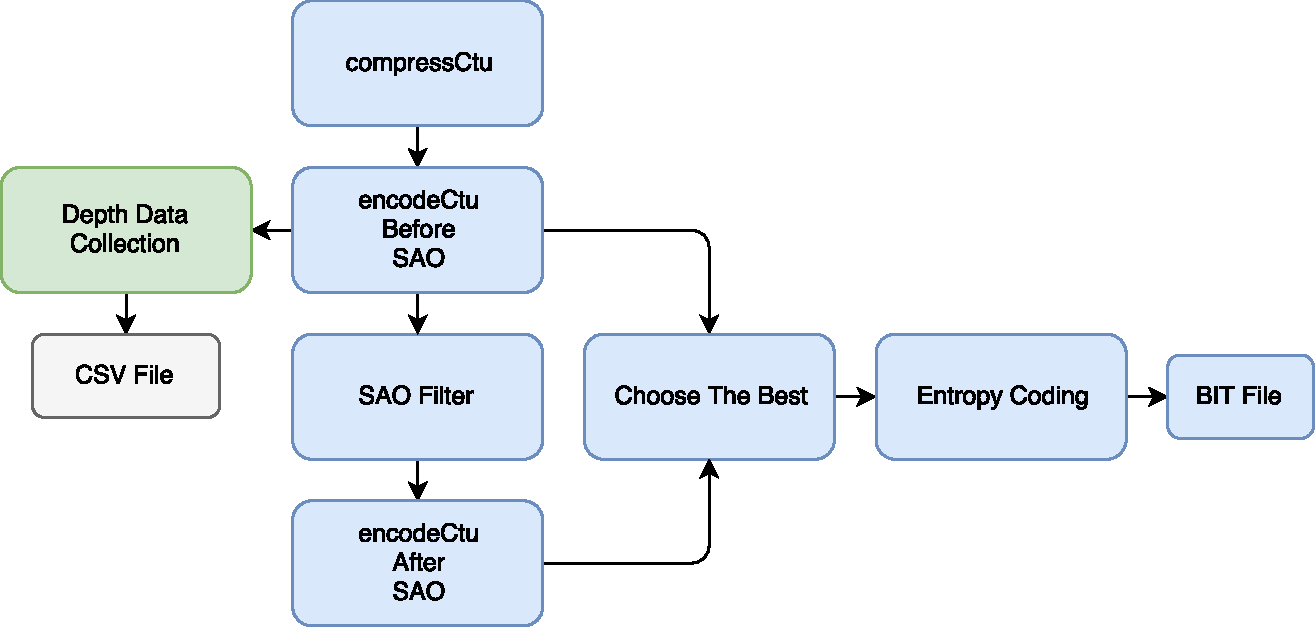
\includegraphics[width=\textwidth,height=\textheight,keepaspectratio]{Figures/thesis-data-collecting-diagram.pdf}
    \caption[Data collecting diagram]{Data collecting diagram.}
    \label{fig:data-collection-diagram}
\end{figure}

During the data collecting process, only Luma samples in depth blocks
are used since we are trying to
reduce the computational complexity of DMM1.
And the luma samples are flattened from rectangle CU blocks into
a single row which will be subsequently written into associated CSV file.
The detailed implementation for the module of \emph{depth data collection}
is shown in Algorithm~\ref{algo:collect-data} on
page~\pageref{algo:collect-data}.
\begin{algorithm}[!t]
    \SetKwData{pcCU}{pcCU}
    \SetKwData{Left}{left}
    \SetKwData{uiAbsPartIdx}{uiAbsPartIdx}
    \SetKwData{uiDepth}{uiDepth}
    \SetKwData{DISFlag}{DISFlag}
    \SetKwData{iPartNum}{iPartNum}
    \SetKwData{sizeOfNByN}{sizeOfNByN}
    \SetKwData{maxCUWidth}{maxCUWidth}
    \SetKwData{pcPic}{pcPic}
    \SetKwData{pcSlice}{pcSlice}
    \SetKwData{pOrg}{pOrg}
    \SetKwData{iStride}{iStride}
    \SetKwData{uiCuSize}{uiCuSize}
    \SetKwData{pOrgPel}{pOrgPel}
    \SetKwData{sizeOfSubBlk}{sizeOfSubBlk}
    \SetKwData{uiTPelY}{uiTPelY}
    \SetKwData{uiLPelX}{uiLPelX}
    \SetKwData{yStartPos}{yStartPos}
    \SetKwData{yEndPos}{yEndPos}
    \SetKwData{xStartPos}{xStartPos}
    \SetKwData{xEndPos}{xEndPos}
    \SetKwData{iDir}{iDir}
    \SetKwData{partitionMode}{partitionMode}
    \SetKwFunction{getCUSize}{getCUSize}
    \SetKwFunction{getSizeOfSubBlk}{getSizeOfSubBlk}
    \SetKwFunction{FindCompress}{FindCompress}
    \SetKwFunction{getIntraDir}{getIntraDir}
    \SetKwFunction{getPic}{getPic}
    \SetKwFunction{getSlice}{getSlice}
    \SetKwFunction{getAddr}{getAddr}
    \SetKwFunction{getStride}{getStride}
    \SetKwFunction{getYPelCU}{getYPelCU}
    \SetKwFunction{getPartitionSize}{getPartitionSize}
    \DontPrintSemicolon % Some LaTeX compilers require you to use \dontprintsemicolon instead
    \KwIn{CU data structure \pcCU,
    absolute partition index of CU \uiAbsPartIdx,
    quad-tree depth \uiDepth}
    \KwOut{Flattened luma pixel values of each block together with
    the index of its best intra mode in each row of the output csv file}
    \Begin{
    \For{each CU in depth maps}{
    \uiCuSize$\leftarrow$\getCUSize{\pcCU, \uiDepth}\;
    \pOrgPel$\leftarrow$\getYPelCU{\pcCU}\;
    \If{\DISFlag $\equiv 0$}{
    %  \partitionMode$\leftarrow$ \getPartitionSize{$Im[i,j-1]$}\;
    \partitionMode$\leftarrow$\getPartitionSize{\pcCU, \uiAbsPartIdx}\;

    \eIf{\partitionMode $\equiv$ \sizeOfNByN}{
    \iPartNum$\leftarrow 4$\;
    }{
    \iPartNum$\leftarrow 1$\;
    }

    \For{$j\leftarrow 0$ \KwTo \iPartNum}{
    $iDir[j]$ $\leftarrow$ \getIntraDir{\pcCU, \uiAbsPartIdx}\;
    }
    \eIf{\iPartNum $\equiv 1$}{
    %      \tcc{collect luma values and the best mode for a single block}
    Create a new csv file, append the value of \uiDepth at the end of the name of the new csv file\;
    \For{$y\leftarrow 0$ \KwTo \uiCuSize}{
    \For{$x\leftarrow 0$ \KwTo \uiCuSize}{
    Write $pOrgPel[x]$ into $row_m$ in csv file\;
    }
    \pOrgPel $\leftarrow$ \pOrgPel + \iStride\;
    }
    Write $iDir[0]$ into the end of $row_m$ in the csv file\;
    }{
    %      \tcc{collect luma values and the best modes for each sub parts}
    Create a new csv file, append the value of (\uiDepth + $1$) at the end of the name of the new csv file\;
    \sizeOfSubBlk$\leftarrow$\getSizeOfSubBlk{\pcCU, \uiDepth}\;
    \For{$j\leftarrow 0$ \KwTo \iPartNum}{
    \uIf{$j\equiv0$}{
    \yStartPos $\leftarrow 0$
    \& \xStartPos $\leftarrow 0$
    \& \yEndPos $\leftarrow$ \sizeOfSubBlk\
    \& \xEndPos $\leftarrow$ \sizeOfSubBlk\;
    }
    \uElseIf{$j\equiv1$}{
    \yStartPos $\leftarrow 0$
    \& \xStartPos $\leftarrow$ \sizeOfSubBlk
    \& \yEndPos $\leftarrow$ \sizeOfSubBlk
    \& \xEndPos $\leftarrow \sizeOfSubBlk \times 2$\;
    }
    \uElseIf{$j\equiv2$}{
    \yStartPos $\leftarrow$ \sizeOfSubBlk
    \& \xStartPos $\leftarrow 0$
    \& \yEndPos $\leftarrow \sizeOfSubBlk \times 2$
    \& \xEndPos $\leftarrow$ \sizeOfSubBlk\;
    }
    \uElseIf{$j\equiv3$}{
    \yStartPos $\leftarrow$ \sizeOfSubBlk
    \& \xStartPos $\leftarrow$ \sizeOfSubBlk
    \& \yEndPos $\leftarrow \sizeOfSubBlk \times 2$
    \& \xEndPos $\leftarrow \sizeOfSubBlk \times 2$\;
    }
    }
    \For{$y\leftarrow$ \yStartPos \KwTo \yEndPos}{
    \For{$x\leftarrow$ \xStartPos \KwTo \xEndPos}{
    %   \For{$y\leftarrow 0$ \KwTo \yEndPos}{
    %        \For{$x\leftarrow 0$ \KwTo \xEndPos}{
    Write $pOrgPel[x]$ into $row_m$ in the csv file\;
    }
    \pOrgPel $\leftarrow$ \pOrgPel+ \iStride\;
    }
    Write $iDir[j]$ into the end of $row_m$ in the csv file\;
    }}}}
 \caption{Collect data}
 \label{algo:collect-data}
\end{algorithm}
The inputs to the data collecting workflow are exactly the inputs to
the module of \emph{encodeCtu}, namely the CU data structure,
the absolute partition index and the corresponding quad-tree depth.
Firstly, the partition mode of the CU is obtained which can further indicate
the partition number to either be one or four.
After that, based on the partition number, the best modes for blocks
are stored into an four dimensional array of integer values within the range
from 0 (inclusive) to 36 (inclusive).
If the partition number is equal to one, which means the current CU has not
been split and it has its own best mode.
The luma pixel samples of this block are collected into a single row in the
CSV file.
In the end of the same row, the best mode of the CU is signaled.
If the partition number is equal to four, which means the current CU has been
split to form four smaller sub-blocks with each sub-block has its
own best mode.
The luma samples for each sub-block are collected into four different rows
in the CSV file with the last value in each row to be the best mode for each
sub-block.
HTM16.2~\parencite{RN214} is used in this work, which is the newest
version of the reference software of 3D-HEVC\@.
Considering we are focusing on the intra prediction,
All-Intra configuration is used.

\section{Data Pre-processing}\label{sec:data-preprocessing}


\section{Data Visualization}\label{sec:data-visu}
Some fake things added again.
%Welcome to this \LaTeX{} Thesis Template, a beautiful and easy to use template for writing a thesis using the \LaTeX{} typesetting system.
%
%If you are writing a thesis (or will be in the future) and its subject is technical or mathematical (though it doesn't have to be), then creating it in \LaTeX{} is highly recommended as a way to make sure you can just get down to the essential writing without having to worry over formatting or wasting time arguing with your word processor.
%
%\LaTeX{} is easily able to~\parencite{RN93} professionally typeset documents that run to hundreds or thousands of pages long. With simple mark-up commands, it automatically sets out the table of contents, margins, page headers and footers and keeps the formatting consistent and beautiful. One of its main strengths is the way it can easily typeset mathematics, even \emph{heavy} mathematics. Even if those equations are the most horribly twisted and most difficult mathematical problems that can only be solved on a super-computer, you can at least count on \LaTeX{} to make them look stunning.
%
%%----------------------------------------------------------------------------------------
%
%\section{Welcome and Thanku}\label{sec:welome}
%Welcome to this \LaTeX{} Thesis Template, a beautiful and easy to use template for writing a thesis using the \LaTeX{} typesetting system.
%
%If you are writing a thesis (or will be in the future) and its subject is technical or mathematical (though it doesn't have to be), then creating it in \LaTeX{} is highly recommended as a way to make sure you can just get down to the essential writing without having to worry over formatting or wasting time arguing with your word processor.
%
%\LaTeX{} is easily able to professionally typeset documents that run to hundreds or thousands of pages long. With simple mark-up commands, it automatically sets out the table of contents, margins, page headers and footers and keeps the formatting consistent and beautiful. One of its main strengths is the way it can easily typeset mathematics, even \emph{heavy} mathematics. Even if those equations are the most horribly twisted and most difficult mathematical problems that can only be solved on a super-computer, you can at least count on \LaTeX{} to make them look stunning.
%
%%----------------------------------------------------------------------------------------
%
%\section{Welcome and ThYou}\label{sec:weome}
%Welcome to this \LaTeX{} Thesis Template~\parencite{Reference1}, a beautiful and easy to use template for writing a thesis using the \LaTeX{} typesetting system.
%
%If you are writing a thesis (or will be in the future) and its subject is technical or mathematical (though it doesn't have to be), then creating it in \LaTeX{} is highly recommended as a way to make sure you can just get down to the essential writing without having to worry over formatting or wasting time arguing with your word processor.
%
%\LaTeX{} is easily able to professionally typeset documents that run to hundreds or thousands of pages long. With simple mark-up commands, it automatically sets out the table of contents, margins, page headers and footers and keeps the formatting consistent and beautiful. One of its main strengths is the way it can easily typeset mathematics, even \emph{heavy} mathematics. Even if those equations are the most horribly twisted and most difficult mathematical problems that can only be solved on a super-computer, you can at least count on \LaTeX{} to make them look stunning.
%
%%----------------------------------------------------------------------------------------
%
%\section{Welcome and Thau}\label{sec:welcoe}
%Welcome to this \LaTeX{} Thesis Template, a beautiful and easy to use template for writing a thesis using the \LaTeX{} typesetting system.
%
%\begin{table}
%
%    \label{tab:treatments}
%    \centering
%%    \begin{tabular}{l l l}
%%        \toprule
%%        \tabhead{Groups} & \tabhead{Treatment X} & \tabhead{Treatment Y} \\
%%        \midrule
%%        1 & 0.2 & 0.8\\
%%        2 & 0.17 & 0.7\\
%%        3 & 0.24 & 0.75\\
%%        4 & 0.68 & 0.3\\
%%        \bottomrule\\
%%    \end{tabular}
%    \begin{tabular}{c r @{.} l}
%        Pi expression       &
%        \multicolumn{2}{c}{Value} \\
%        \hline
%        $\pi$               & 3&1416  \\
%        $\pi^{\pi}$         & 36&46   \\
%        $(\pi^{\pi})^{\pi}$ & 80662&7 \\
%    \end{tabular}
%    \caption{The effects of treatments X and Y on the four groups studied.}
%\end{table}
%writing a thesis (or will be in the future) and its subject is technical or mathematical (though it doesn't have to be), then creating it in \LaTeX{} is highly recommended as a way to make sure you can just get down to the essential writing without having to worry over formatting or wasting time arguing with your word processor.
%
%\LaTeX{} is easily able to professionally typeset documents that run to hundreds or thousands of pages long. With simple mark-up commands, it automatically sets out the table of contents, margins, page headers and footers and keeps the formatting consistent and beautiful. One of its main strengths is the way it can easily typeset mathematics, even \emph{heavy} mathematics. Even if those equations are the most horribly twisted and most difficult mathematical problems that can only be solved on a super-computer, you can at least count on \LaTeX{} to make them look stunning.
%
%\section{Welcome and Tnk You}\label{sec:wlcome}
%Welcome to this \LaTeX{} Thesis Template, a beautiful and easy to use template for writing a thesis using the \LaTeX{} typesetting system.
%
%If you are writing a thesis.
%
%%\begin{verbatim}
%\begin{figure}
%    \centering
%    
\includegraphics{Figures/Electron}
%    %    \decoRule
%    \caption[An Electron]{An electron (artist's impression).}
%    \label{fig:Electron}
%\end{figure}
%%\end{verbatim}
%(or will be in the future) and its subject is technical or mathematical (though it doesn't have to be), then creating it in \LaTeX{} is highly recommended as a way to make sure you can just get down to the essential writing without having to worry over formatting or wasting time arguing with your word processor.
%
%\LaTeX{} is easily able to professionally typeset documents that run to hundreds or thousands of pages long. With simple mark-up commands, it automatically sets out the table of contents, margins, page headers and footers and keeps the formatting consistent and beautiful. One of its main strengths is the way it can easily typeset mathematics, even \emph{heavy} mathematics. Even if those equations are the most horribly twisted and most difficult mathematical problems that can only be solved on a super-computer, you can at least count on \LaTeX{} to make them look stunning.
%
%%----------------------------------------------------------------------------------------
    % !TEX root = ../main.tex
\chapter{Train the Deep Model for Prediction}\label{ch:chapter4} % For referencing the chapter elsewhere, use \ref{Chapter1}
%
%%----------------------------------------------------------------------------------------
The convolutional neural networks (CNNs) consist of neurons that have 
weights and bias, which can be trained using large datasets for solving 
computer vision tasks.
In this chapter, our architecture of
deep convolutional neural network for intra mode prediction 
is illustrated.
Then the hyper-parameters of our deep model is introduced
with explanations.
At the end of the chapter, the stopping criteria and training results 
are presented.
\begin{figure}
    \centering
    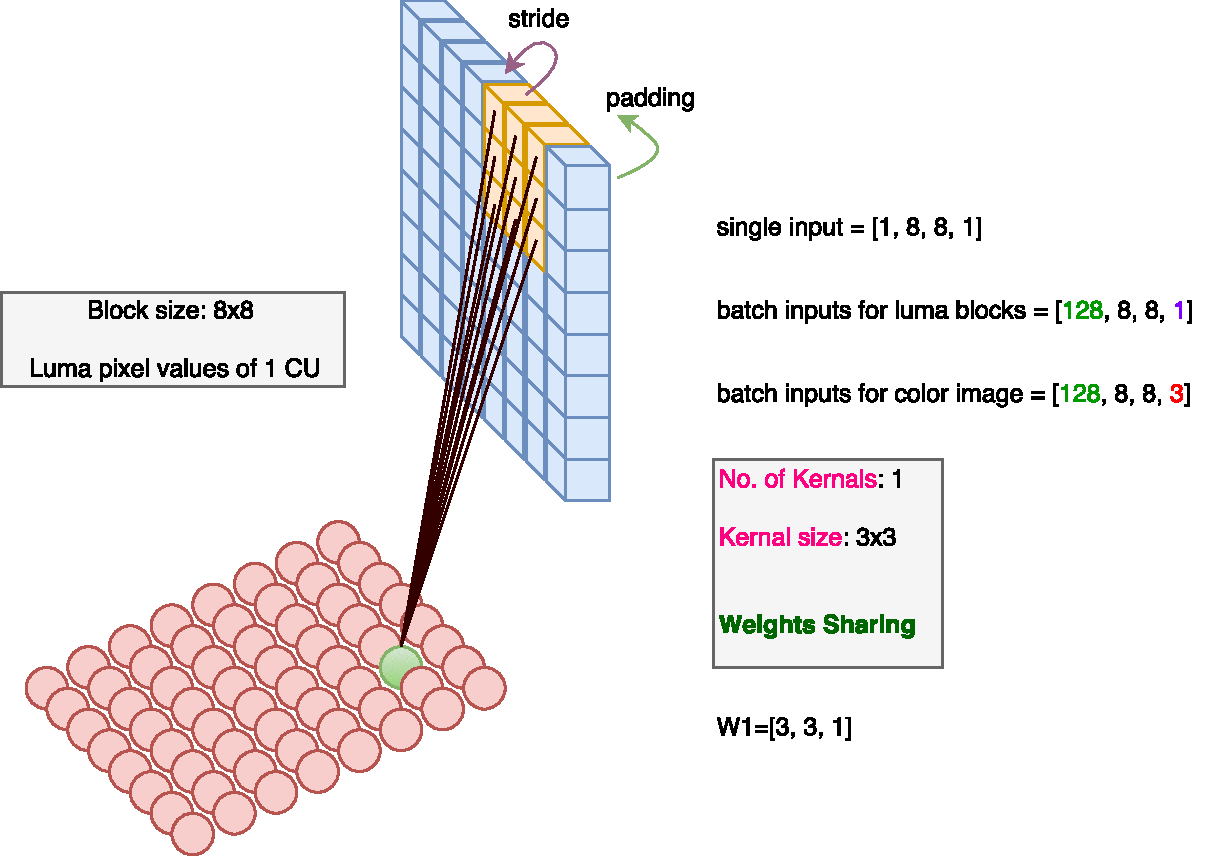
\includegraphics[width=\textwidth,height=\textheight,keepaspectratio]{Figures/cnn_illustration.pdf}
    \caption[Two types of the residual units]{
        Two types of the residual units.}\label{fig:cnn-illustration}
\end{figure}

\section{The Architecture of CNN}\label{sec:cnn}
There exist many kinds of convolutional neural networks while the 
major difference that distinguish them from each other
is the uniqueness of each architecure.
Figure~\ref{fig:cnn-illustration} on 
page~\pageref{fig:cnn-illustration}
illustrates the basic architecture
of the convolutional neural networks.
The light blue cubics represent the Luma pixel values from a single
coding unit (CU) of size \(8\times8\) while the yellow cubics
shows a kernel of size \(3\times3\) that slides over the
CU in both directions.
At each position, the kernel does a weighted sum of all its inputs,
then adds biases. The output from the
region it covers will be fed into a neuron right 
below the covered region.
Although both are artificial neural networks, 
the big difference between multilayer perceptron and 
CNN is that weights of the neurons are shared in the latter case.
For example, all the neurons in Figure~\ref{fig:cnn-illustration} on
page~\pageref{fig:cnn-illustration} are reusing the same patch of
parameters, i.e., weights and biases.
For a single kernal of size \(3\times3\), it has 9 weights.
Apparently this amount of learnable parameters is just not enough.
More degrees of freedom are needed to enable 
the learning capability of a neural network.
For this reason, multiple kernels will be used instead of one single kernal.
If many kernels are stacked in a convolutional neural network such that
the architecture looks very deep, the network is called deep neural network
instead of simply neural network which typically refers to shallow ones.
In the deep convolutional neural networks, it can be imagined that
each convolutional layer comprising multiple kernels which subsequently produces
a three dimensional volume of the outputs.
After the convolutional layer, there normally exist activating layer where
the specified activation function will be applied to each single output
inside the output volume from the convolutional layer.
Followed by the activating layer, there is a pooling layer.
In the previous years, the maximum pooling and average pooling 
are popular methods for reducing the dimension of the outputs
from convolutional layers.
Nowadays, instead of applying a conventional pooling, 
a convolutional layer of larger stride is utilized.
Such a combination of convolution-activation-pooling will
be replicated multiple times for a single convolutional neural network.
In the tail of the network, a fully-connected layer can be used
to compute the probability of each target class for the 
classification problems.

Our network is built from the above description except the 
fact that we have adopted the identity mapping 
\(h(\mathbf{x}_l)=\mathbf{x}_l\) in the Residual 
Neural Network from~\parencite{RN67}.
It has been shown in~\parencite{RN68} that
the identity mapping in the residual units
can enable the direct propagation of information
from one layer to any other layers.
Such a nice property brings vital benefits
for deep neural networks such that the accuracy
saturation problem can be alleviated.
As a result, ultra-deep models are able to
learn desired representations for solving
problems.
Besides, with the identity mapping, the network
is able to converge faster hence the training time
required for a deep model can be reduced.
% The architecture of the deep 
Figure~\ref{fig:basic-resnet-structure} on 
page~\pageref{fig:basic-resnet-structure}
shows two types
of the residual units which implement the identity mapping
via shortcut connections from the beginning of the block
to the end of the same block.
\begin{figure}
    \centering
    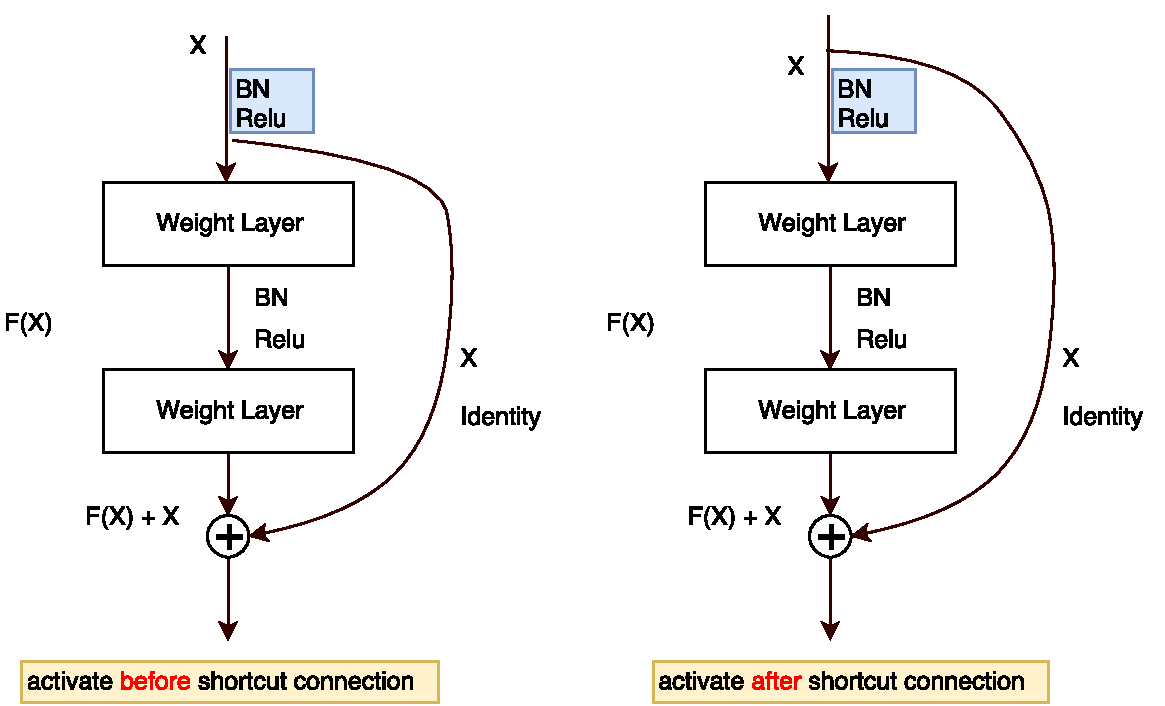
\includegraphics[width=\textwidth,height=\textheight,keepaspectratio]{Figures/basic-resnet-structure.pdf}
    \caption[Two types of the residual units]{
        Two types of the residual units are shown here.
        BN stands for Batch Normalization while
        Relu stands for Rectified Linear Unit.
        }\label{fig:basic-resnet-structure}
\end{figure}

The architecture of the deep convolutional neural 
network used for intra mode prediction in our work
is shown in Figure~\ref{fig:our-architecture} on
page~\pageref{fig:our-architecture}.
The first layer consists of 16 kernels where
the receptive fields are 
simply stacked on top of each other.
In the middle of the network, there are
three variants of resnet unit, each unit
is duplicated five times to deepen the network
for more learning capacities.
Batch Normalization is employed to regularize
the data inputs as well as the outputs from each layer.
The activation function is the most popular one named Relu.
In the end of the convolutional layers, global average pooling
has been performed before the fully-connected layer which 
tells the prediction results.


\begin{figure}
    \centering
    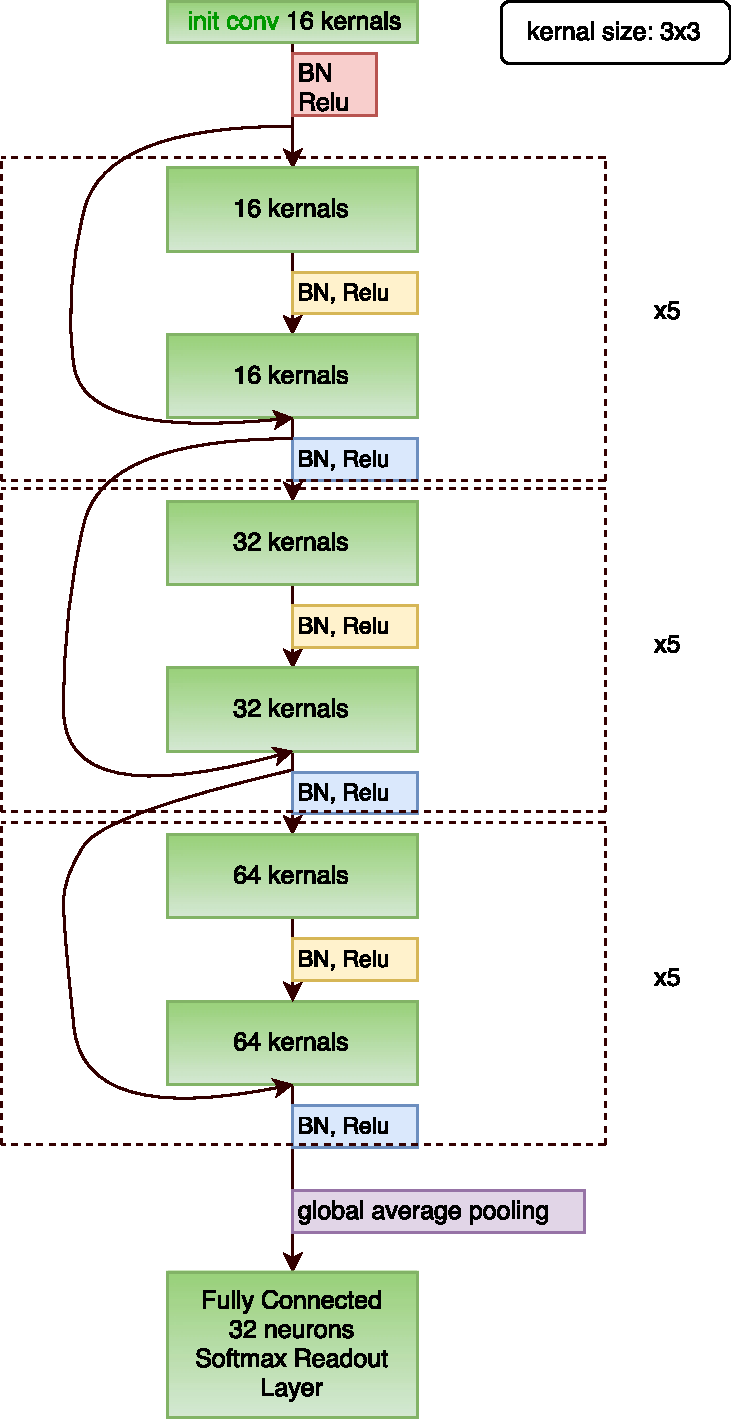
\includegraphics[width=\textwidth,height=\textheight,keepaspectratio]{Figures/our-neural-net-structure.pdf}
    \caption[Top-20 precision on validation dataset for blocks of size \(4\times4\)]{
        Top-20 precision on validation dataset for blocks of size \(4\times4\).
        }\label{fig:our-architecture}
\end{figure}

\section{Settings of the Network}\label{sec:config}
In this section, the hyper-parameters that are
used for deep learning are given.
The configurations are fine-tuned results against the validation
datasets shown in Table~\ref{tab:finalized-eight-by-eight}
and Table~\ref{tab:finalized-sixteen-by-sixteen} to achieve the
best performance.

It is interesting to notice that inside this network, 
the size of any reception field
is always \(3\times3\) since it is found in~\parencite{RN62}
larger kernel can be factorized into smaller kernels.
A kernal with such a size is the smallest
field which is capable of capturing the positional
information~\parencite{RN107}.
All the strides are set to be one which means
no down-sampling will be performed. 
Hence the output size of each convolutional layer
will not be changed.
% The network configuration is shown in Table~\ref{tab:xxxx}.
For the inputs to the convolutional layers, 
zero padding (a.k.a\ SAME padding) is used.
It is a padding algorithm which has the objective
to pad zeros evenly for each direction.
No data augmentation is used for the inputs.
The kernal parameters are randomly initialized 
with a normal distribution where the mean 
is zero while the standard deviation is 
calculated using 
\(\sqrt{2\div(\mathit{a}\times\mathit{a}\times\mathit{n})}\).
Here the \(\mathit{a}\) represents the kernel size
while \(\mathit{n}\) denotes the number of filters
in the corresponding convolutional layer.
The weights of the kernels are regularized by
a decay of \(0.0002\).
No transfer learning is used which means all the learnable 
parameters are trained from scratch.
The batch size used for training is 128.
The loss function used is cross-entropy which has
a better performance for classification problems 
than other distance functions such as L1 and L2.
Stochastic gradient descent is used with a momentum 
of \(0.9\).
The learning rate decay policy is shown in 
Table~\ref{tab:lr-policy}.

\begin{table}[H]
    \caption{Learning rate policy}
    \bigskip\label{tab:lr-policy}
    \centering
    \begin{tabular}{c c}
        \toprule
        Global step & Learning rate \\
        \midrule
        \(<\)20,000 & 0.01 \\
        \(<\)40,000 & 0.001 \\
        \(<\)60,000 & 0.0001 \\
        Others  & 0.00001 \\
        \bottomrule
    \end{tabular}
\end{table}

\section{Stopping Criteria and Training Result}\label{sec:training}
During the training process, we keep eyes on 
various statistics to ensure the network is
truly learning high dimensional representations 
instead of being trapped
in an undesired status where nothing can be
learned.
Tensorflow~\parencite{tensorflow2015-whitepaper} has 
been used in this work to implement the 
deep convolutional neural network.
It has its own dedicated suite of visualization
tools named Tensorboard which is very helpful 
with understanding and monitoring the training process.
It has been configured to record the top-k precision
on the validation datasets during our training process.

Figure~\ref{fig:top20for4times4} 
on page~\pageref{fig:top20for4times4}
is a screen capture
of the Tensorboard user interface which contains the 
top-20 validation precision for blocks of size \(4\times4\).
It can be seem that top-20 precision cannot go 
beyond \(0.85\).
Figure~\ref{fig:top28for4times4}
on page~\pageref{fig:top28for4times4}
further shows the 
top-28 validation precision for blocks of the same size.
Although the highest precision can reach \(0.96\) 
in Figure~\ref{fig:top28for4times4}, it is not applicable
in our case since it involves 28 classes to achieve this 
acceptable precision.
Only four classes would be excluded.
Due to this observation, it is decided to
keep the intra mode decision process unmodified for 
blocks of size \(4\times4\) in \(HTM16.2\).

Figure~\ref{fig:top16for8times8}
on page~\pageref{fig:top16for8times8}
shows the 
top-16 validation precision for blocks of size \(8\times8\).
After 133k global steps, the top-16 precision curve in 
Figure~\ref{fig:top16for8times8} is very steady.
The precision value is higher than \(0.92\).
It means if this model can be employed to predict the 
most probable intra angular directions,
half of the angular directions can be skipped for
the Rate Distortion Cost evaluation process by which
a bunch of time shall be saved.
Figure~\ref{fig:top16for16times16} 
on page~\pageref{fig:top16for16times16}
shows the
top-16 validation precision for blocks 
of size \(16\times16\).
After 304k global steps, the top-16 precision in
Figure~\ref{fig:top16for16times16} has reached
\(0.9654\) which is considered as an excellent
result in our application scenario.
Once again, the half of the intra angular modes
can be bypassed if this model can be applied 
in \(HTM16.2\).
For the blocks of size \(32\times32\),
the dataset obtained for them does not 
have enough data
for the deep learning.
Instead of using a dedicated model for them,
the model trained from blocks of 
size \(16\times16\) has been reused.
The blocks of size \(32\times32\) are resized
to \(16\times16\) using Bilinear Interpolation.

Apart from observing the validation precision,
confusion matrix is the other useful criteria 
to help making decision on when to stop the 
training.
Figure~\ref{fig:cm8times8}
on page~\pageref{fig:cm8times8} shows the confusion
matrix after 173 epochs of training for blocks
of size \(8\times8\).
Figure~\ref{fig:cm16times16}
on page~\pageref{fig:cm16times16} shows the confusion
matrix after 396 epochs of training for blocks
of size \(16\times16\).
Both of the two confusion matrices exhibit
good property which shows most of the predictions
fall in the top-k predictions.

\begin{figure}
    \begin{minipage}{0.98\textwidth}
    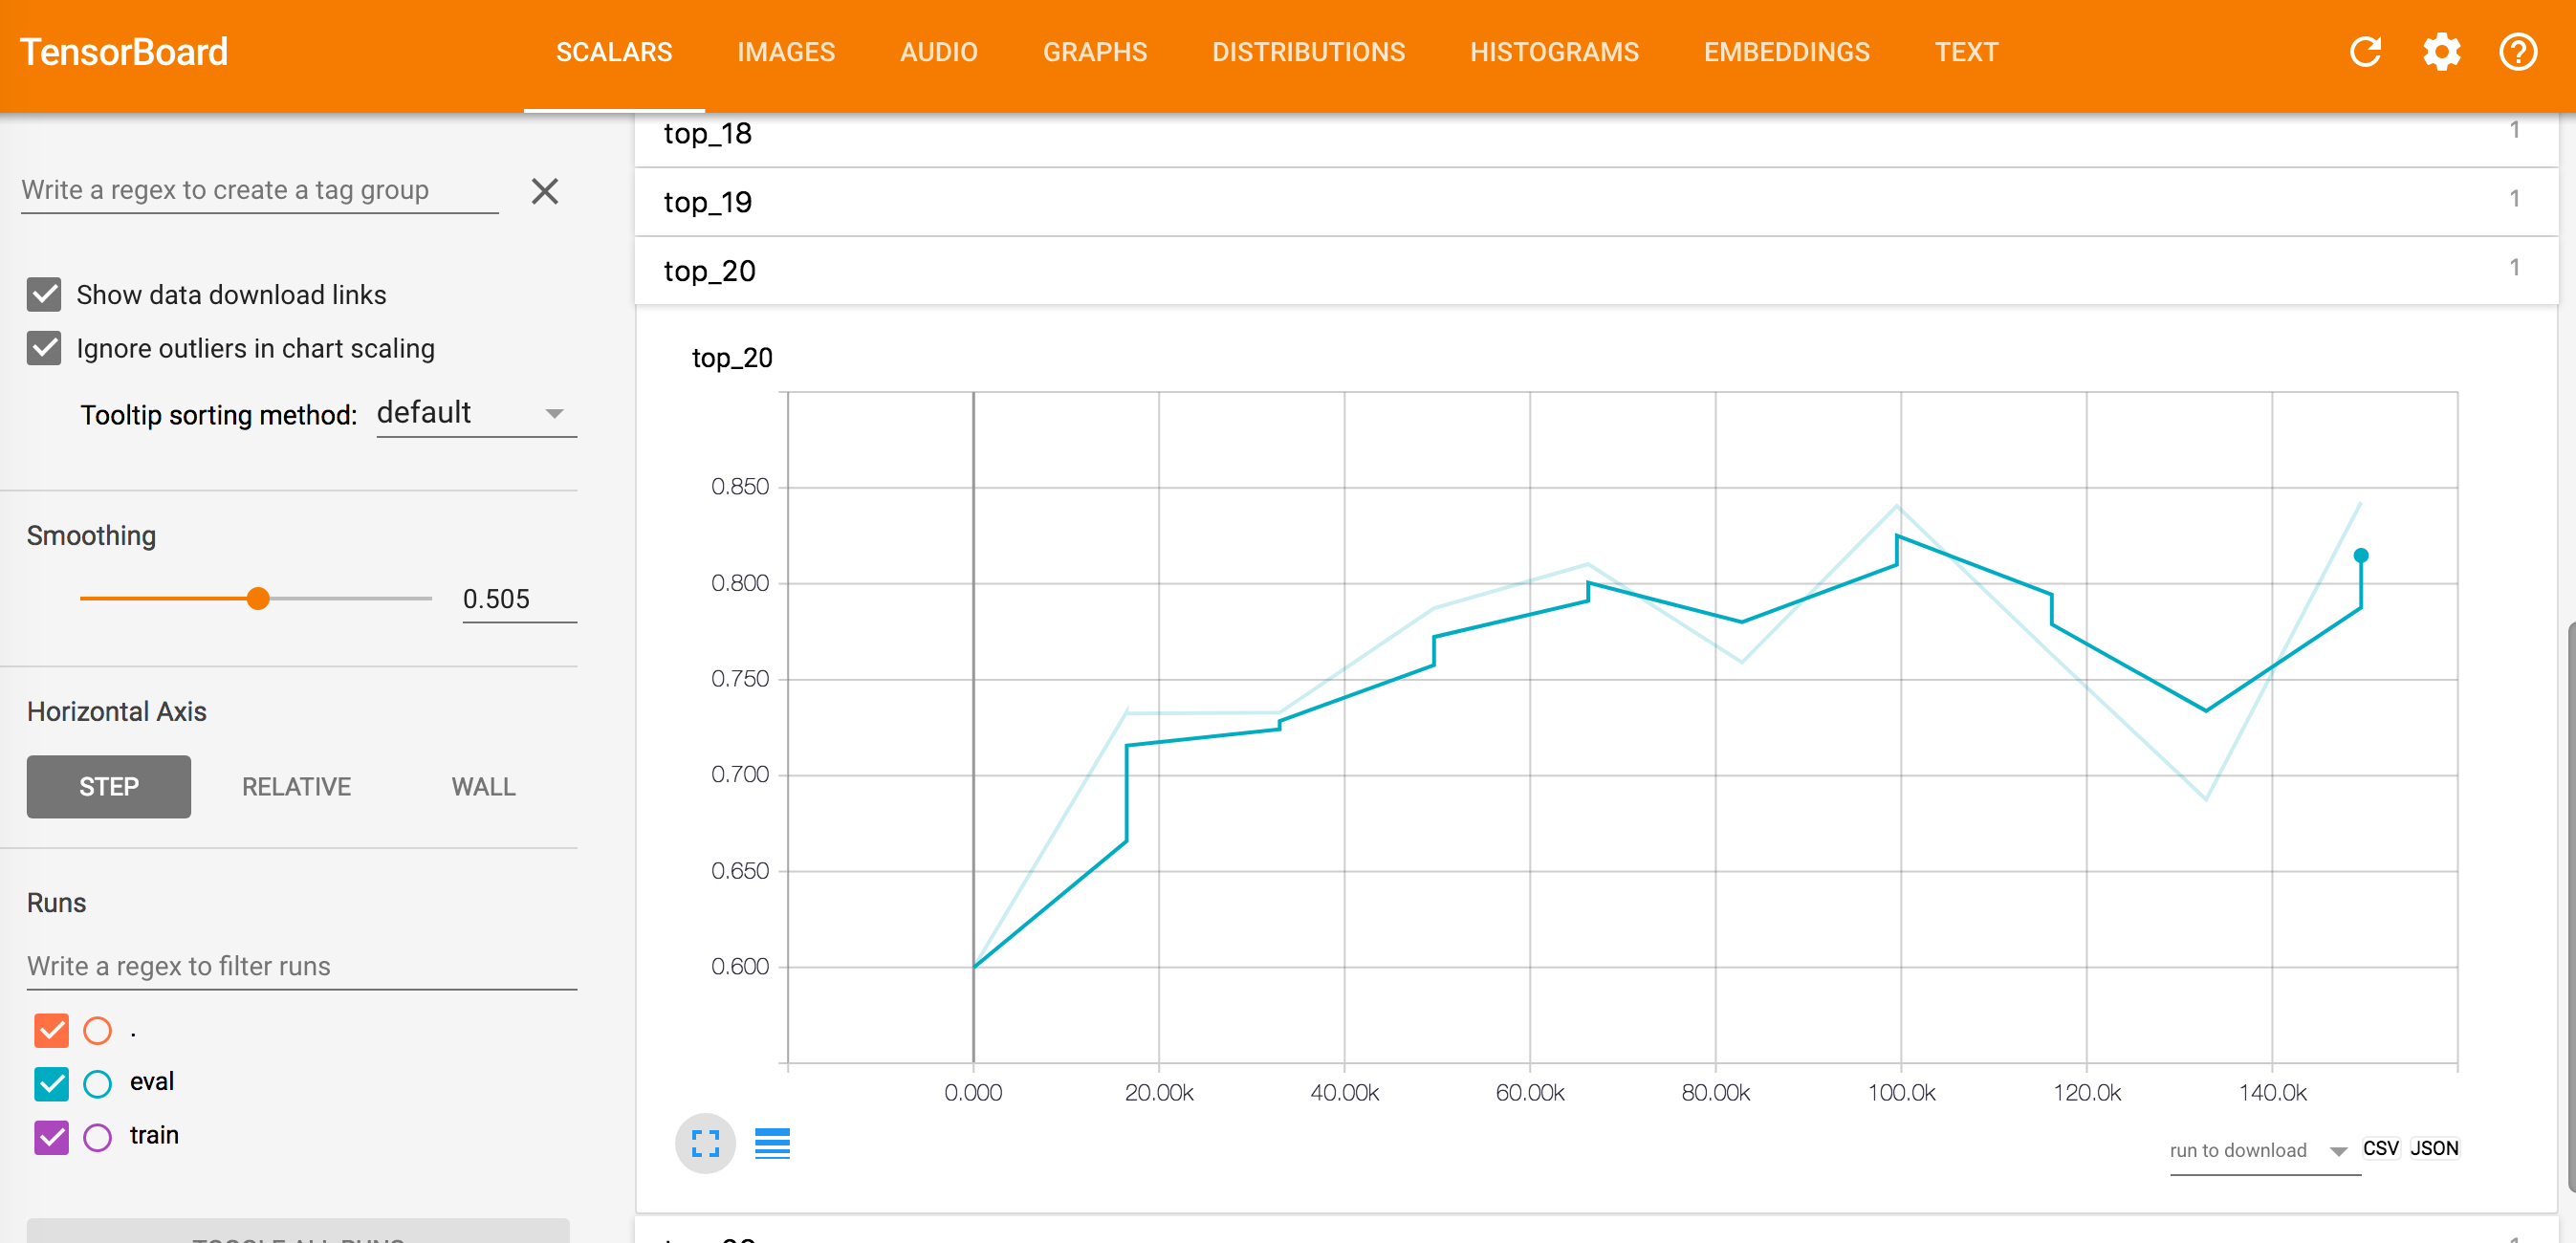
\includegraphics[width=\textwidth,height=\textheight,keepaspectratio]{Figures/blk-4--top-20.png}
    \caption[Top-20 precision on validation dataset for blocks of size \(4\times4\)]{
        Top-20 precision on validation dataset for blocks of size \(4\times4\).
        }\label{fig:top20for4times4}
    \end{minipage}
    
    \vspace*{1cm} % vertical separation

    \begin{minipage}{0.98\textwidth}
    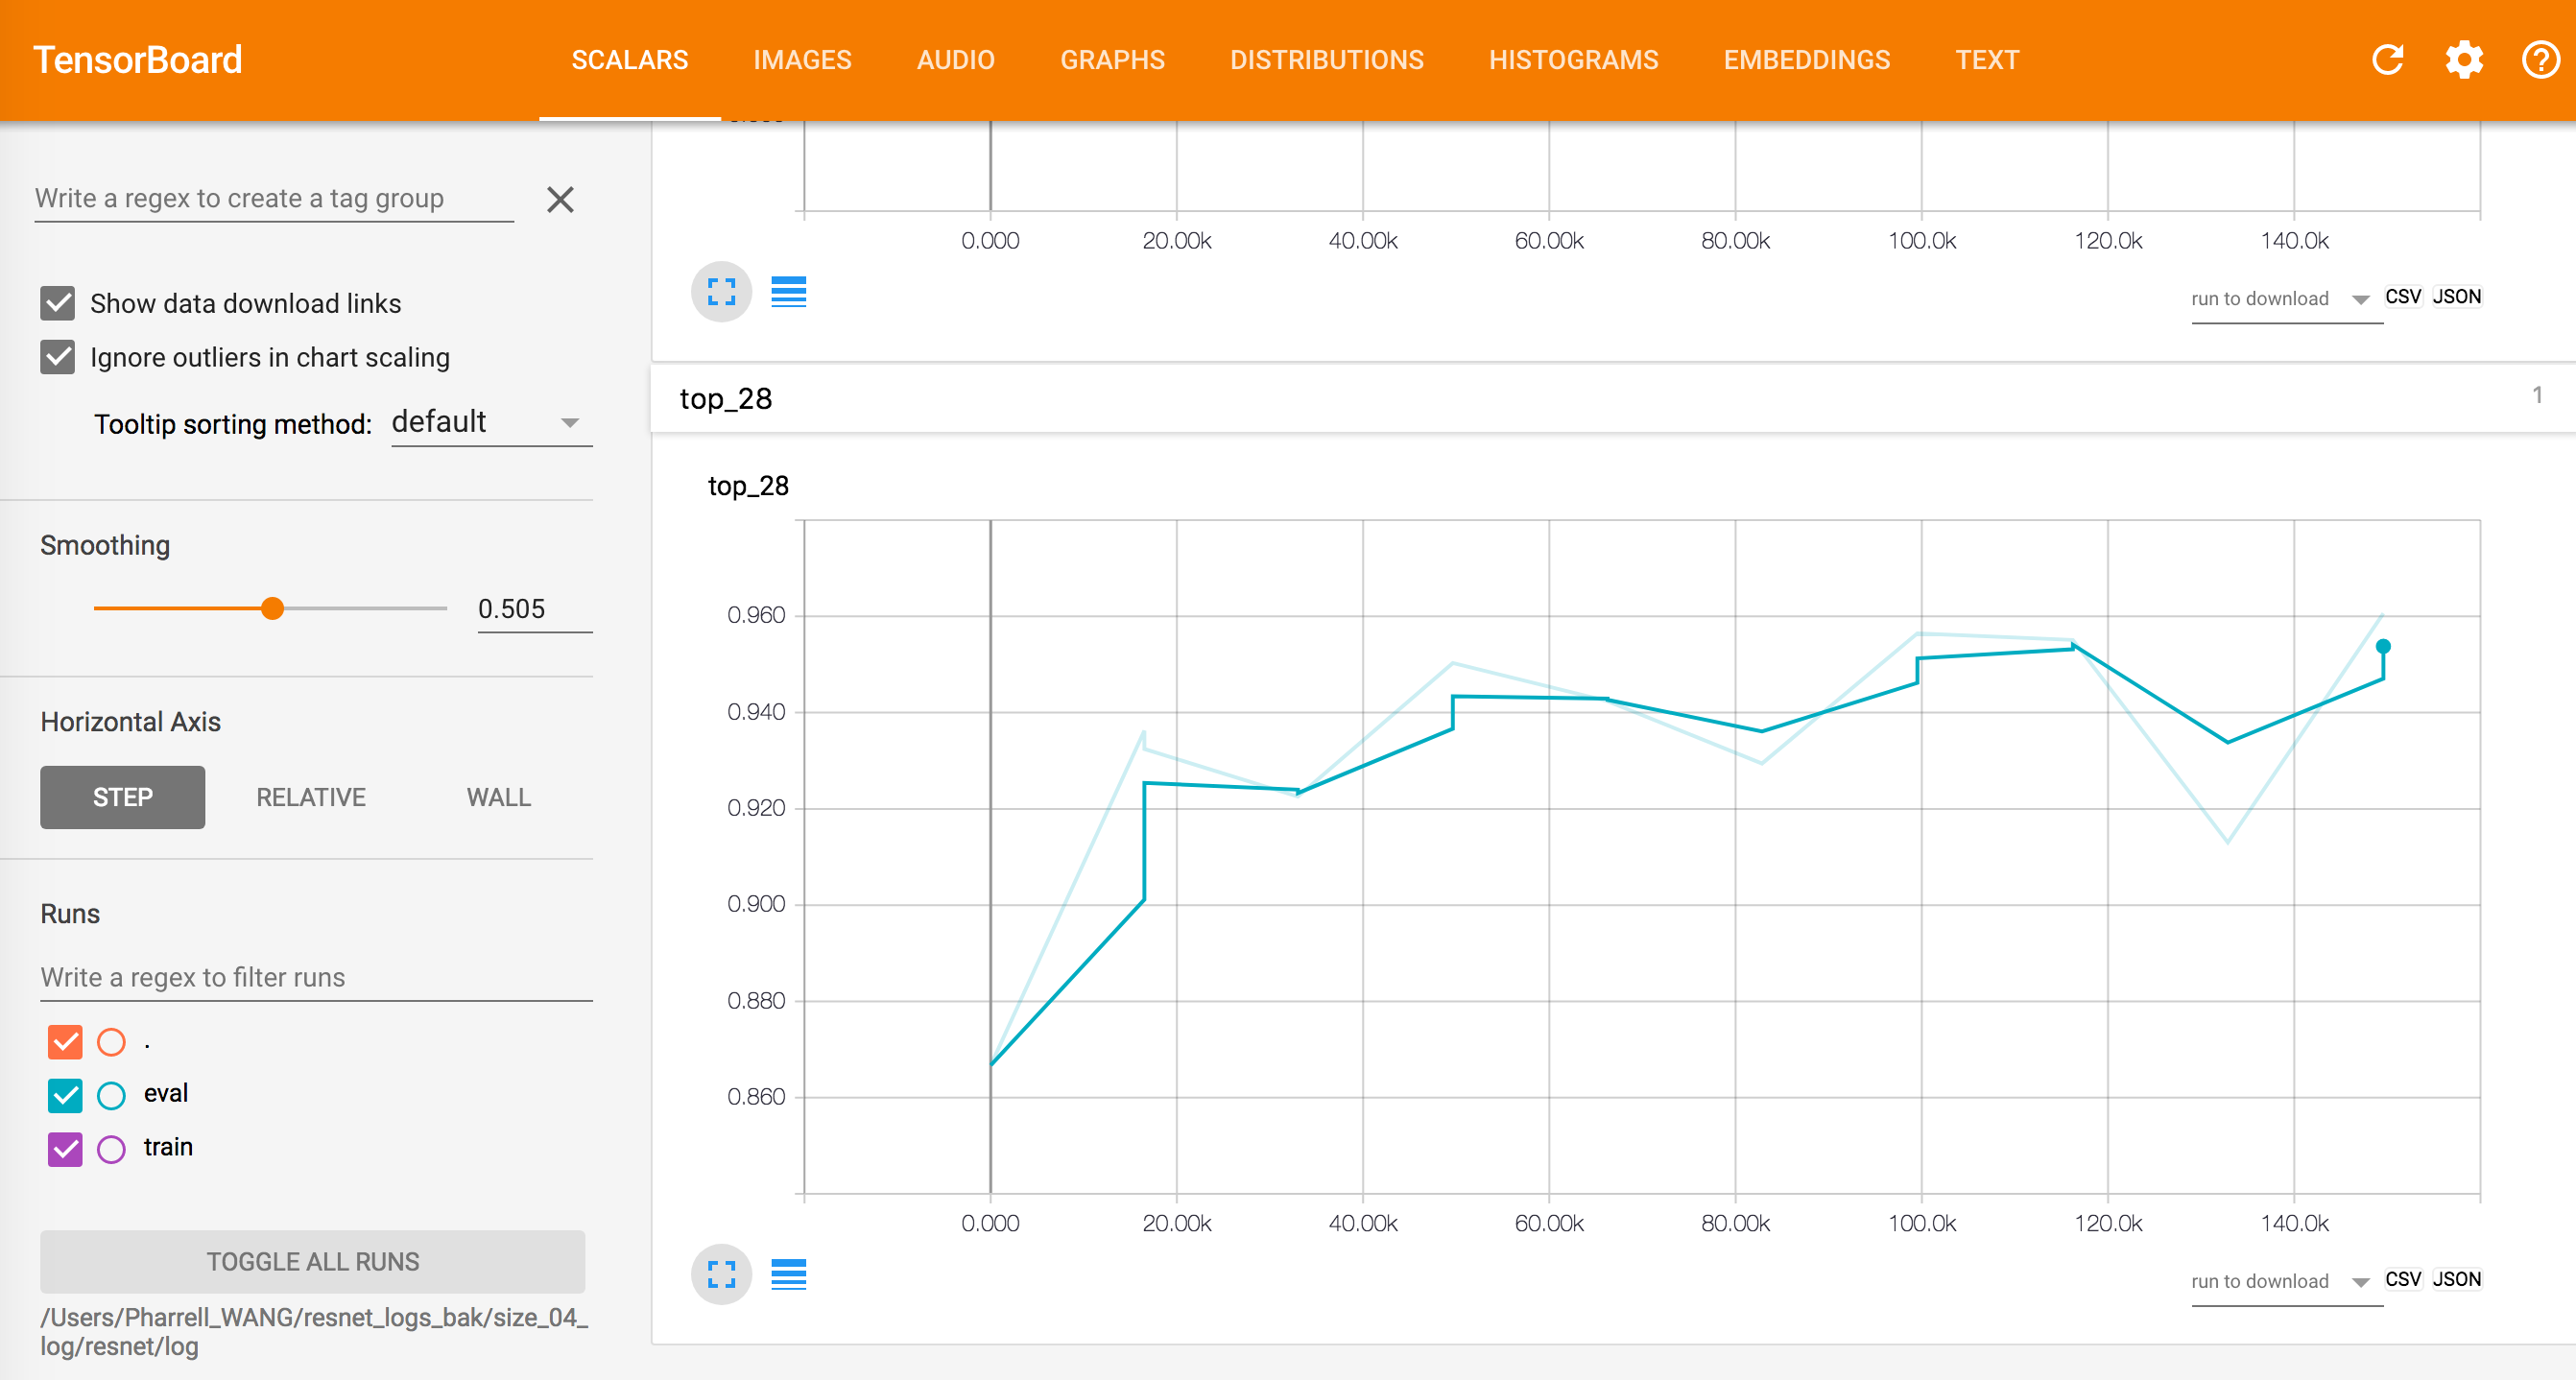
\includegraphics[width=\textwidth,height=\textheight,keepaspectratio]{Figures/blk-4--top-28.png}
    \caption[Top-28 precision on validation dataset for blocks of size \(4\times4\)]{
        Top-28 precision on validation dataset for blocks of size \(4\times4\).
        }\label{fig:top28for4times4}
    \end{minipage}
\end{figure}

\begin{figure}
    \begin{minipage}{0.98\textwidth}
    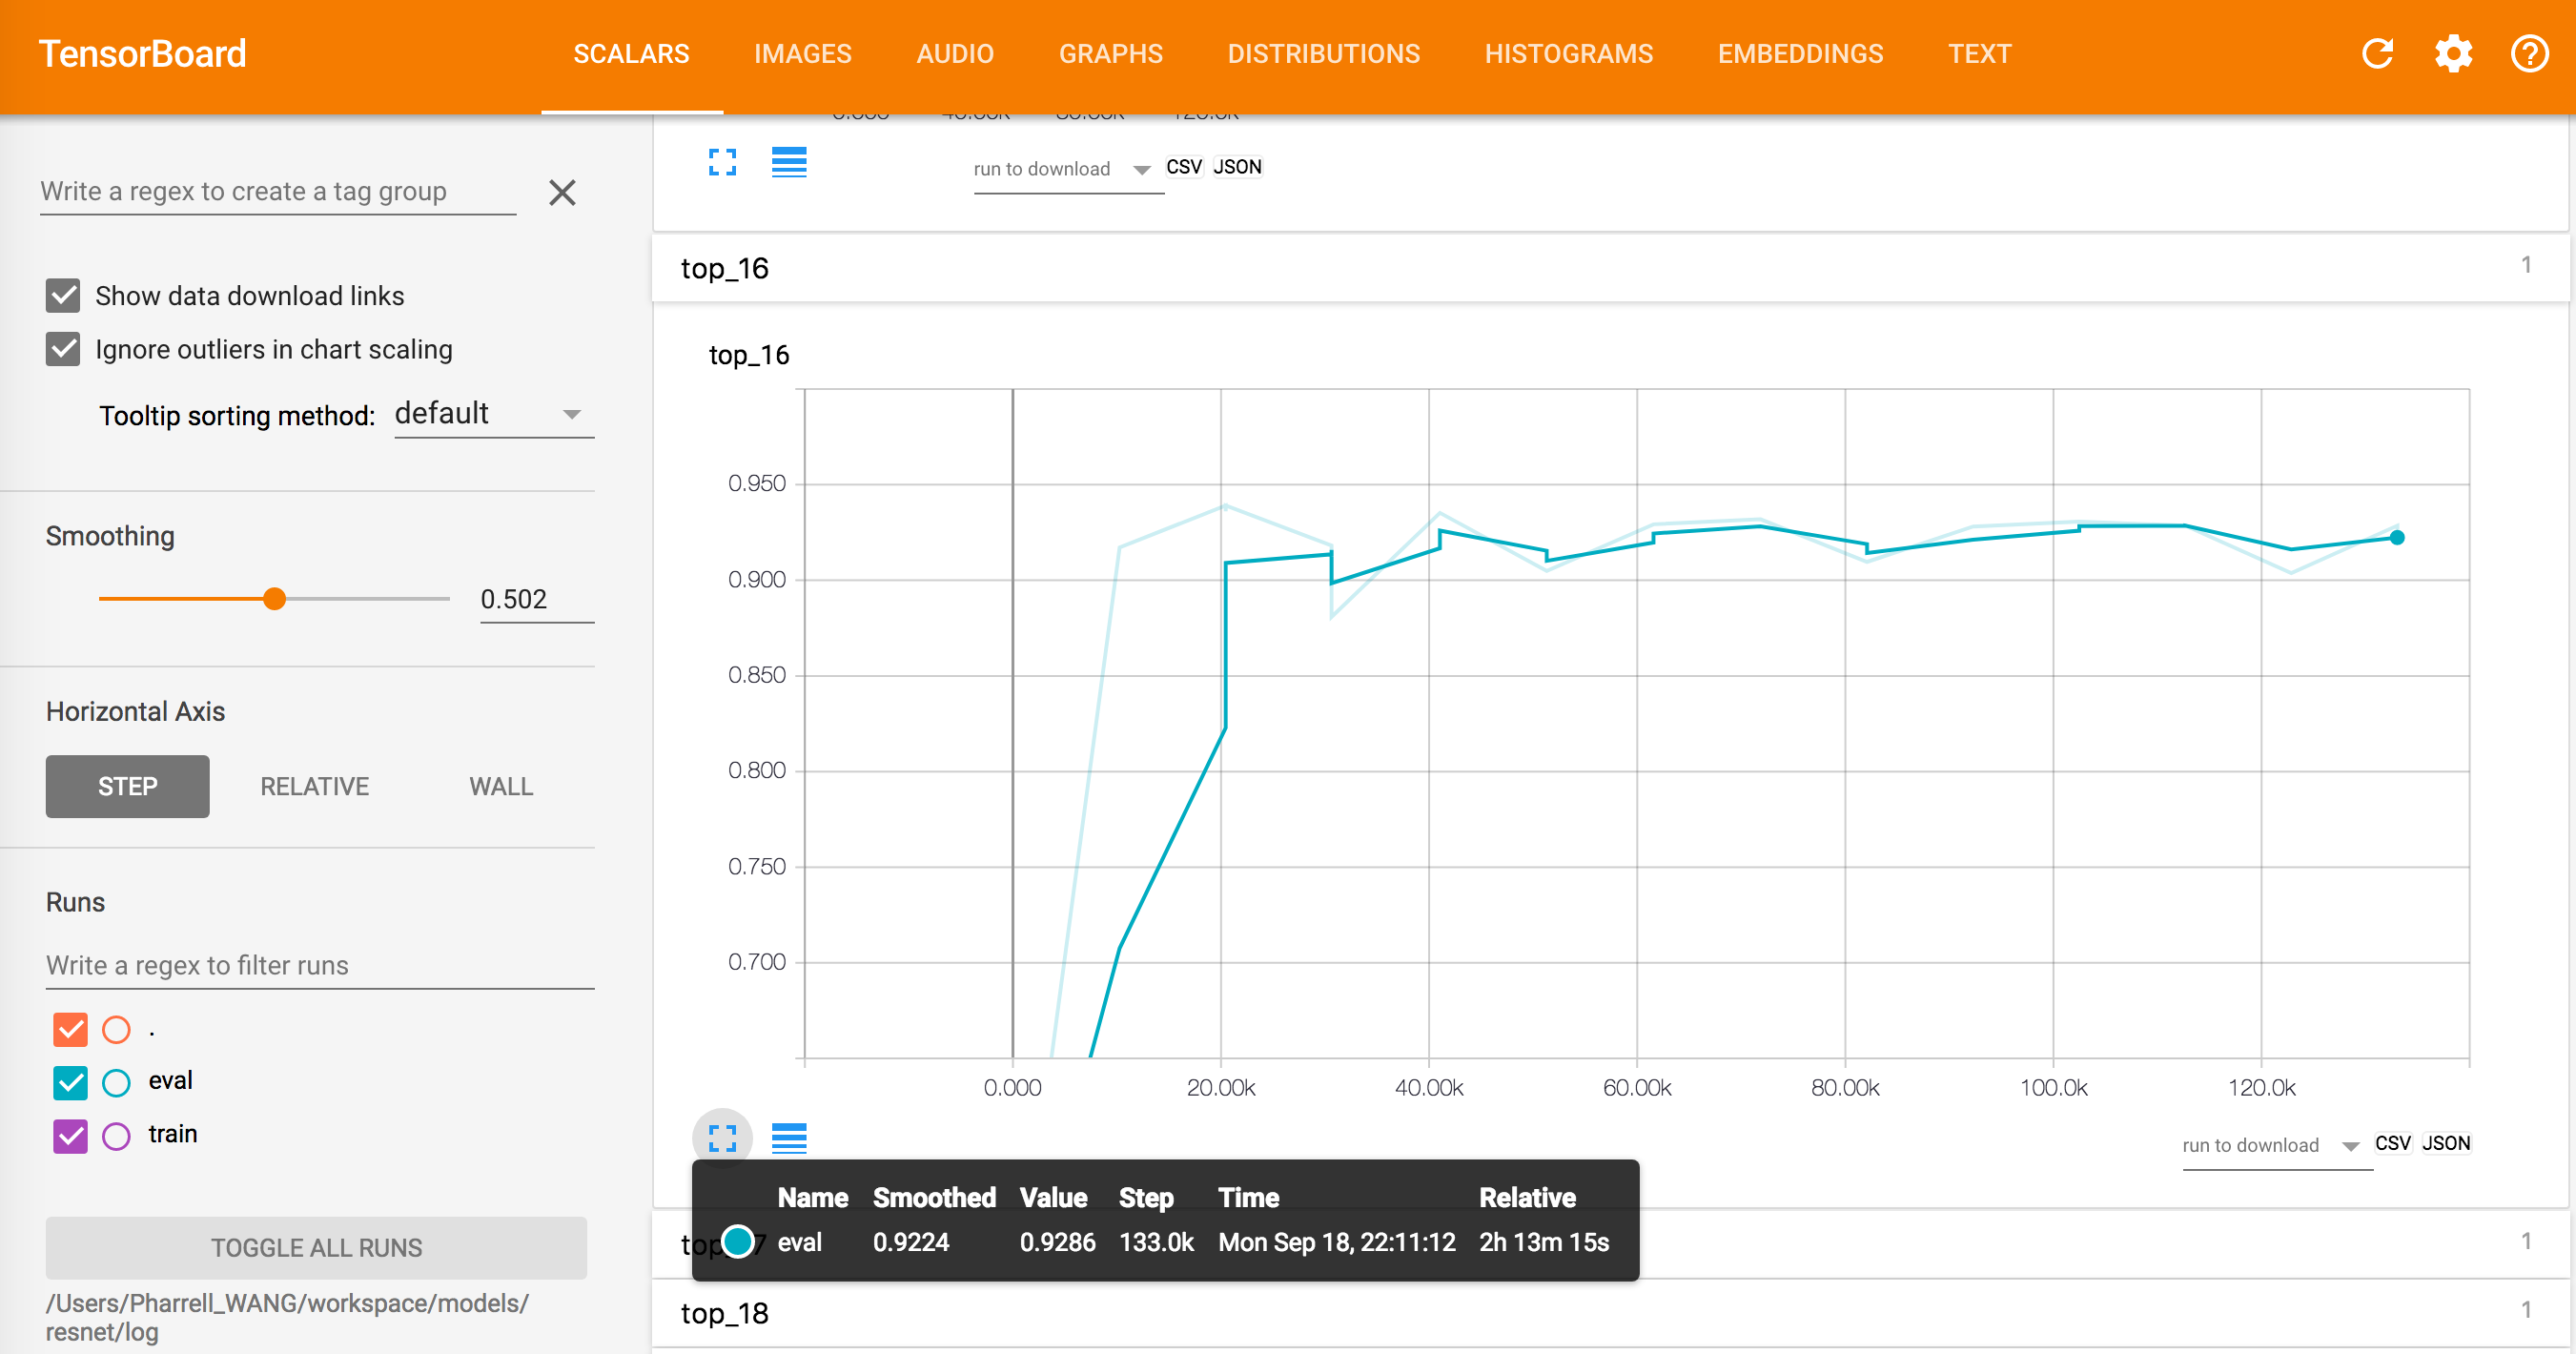
\includegraphics[width=\textwidth,height=\textheight,keepaspectratio]{Figures/blk-8--top-16.png}
    \caption[Top-16 precision on validation dataset for blocks of size \(8\times8\)]{
        Top-16 precision on validation dataset for blocks of size \(8\times8\).
        }\label{fig:top16for8times8}
    \end{minipage}
    
    \vspace*{1cm} % vertical separation

    \begin{minipage}{0.98\textwidth}
    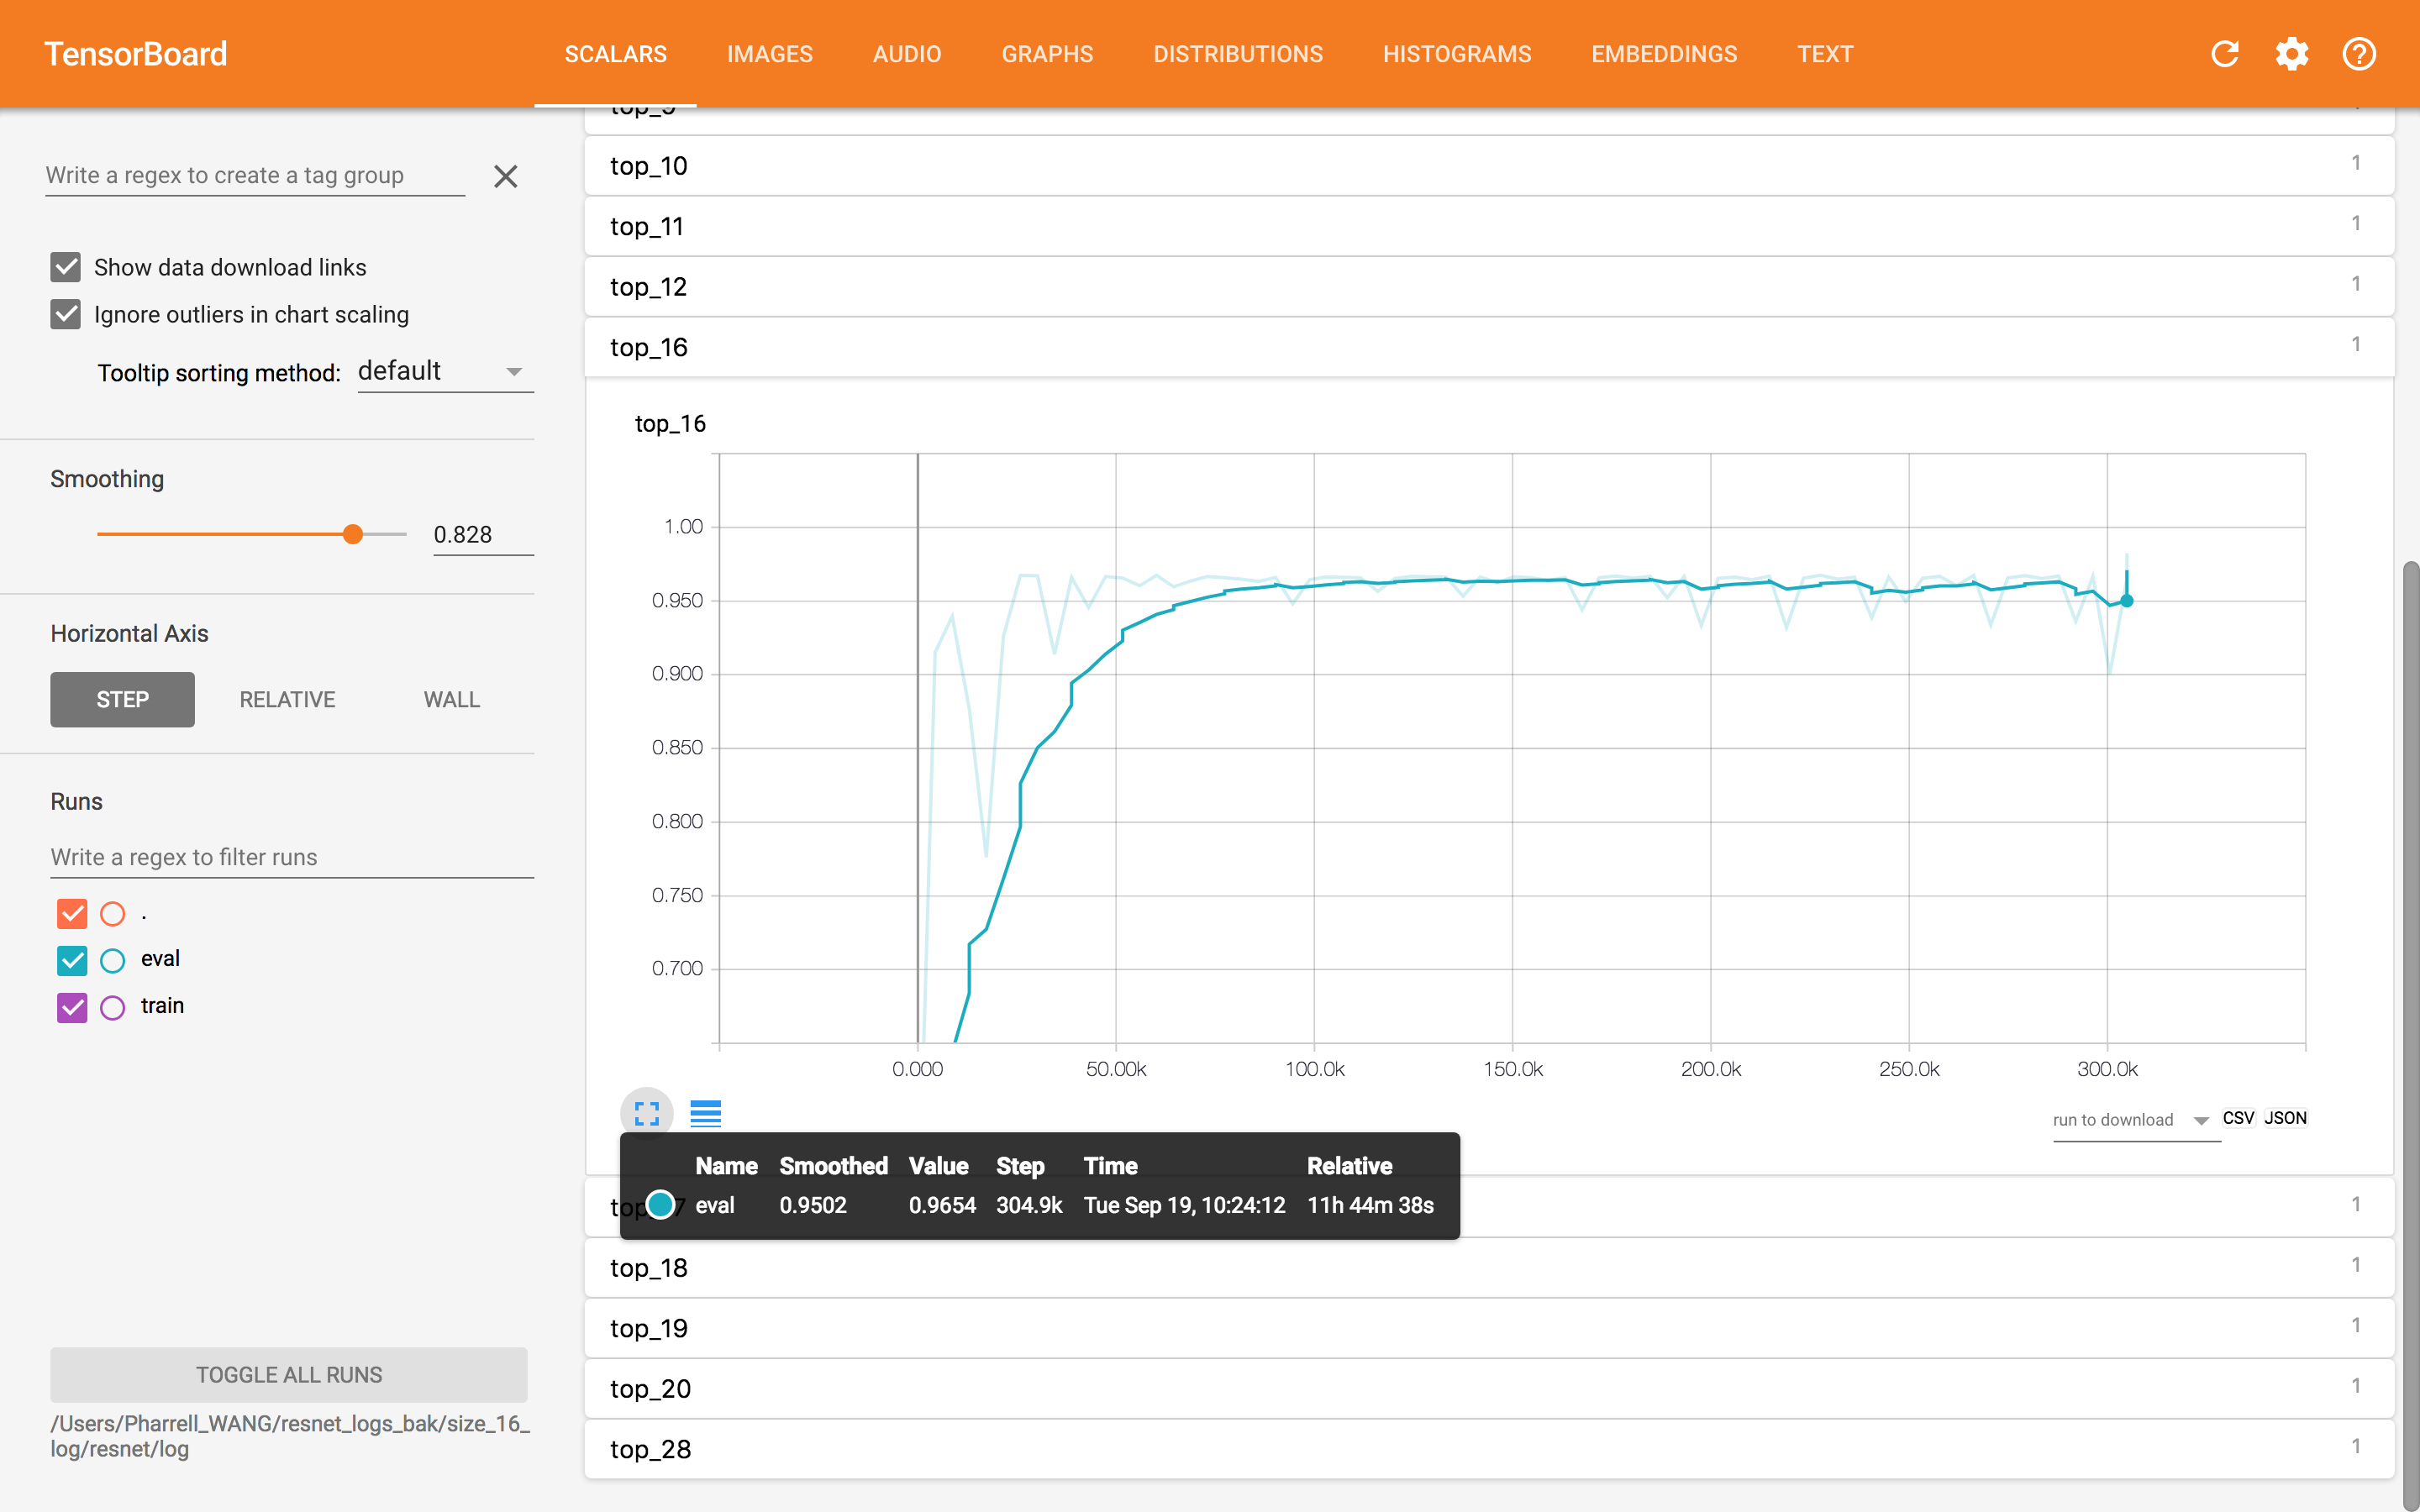
\includegraphics[width=\textwidth,height=\textheight,keepaspectratio]{Figures/blk16-top16.png}
    \caption[Top-16 precision on validation dataset for blocks of size \(16\times16\)]{
        Top-16 precision on validation dataset for blocks of size \(16\times16\).
        }\label{fig:top16for16times16}
    \end{minipage}
\end{figure}

\begin{figure}
    \centering
    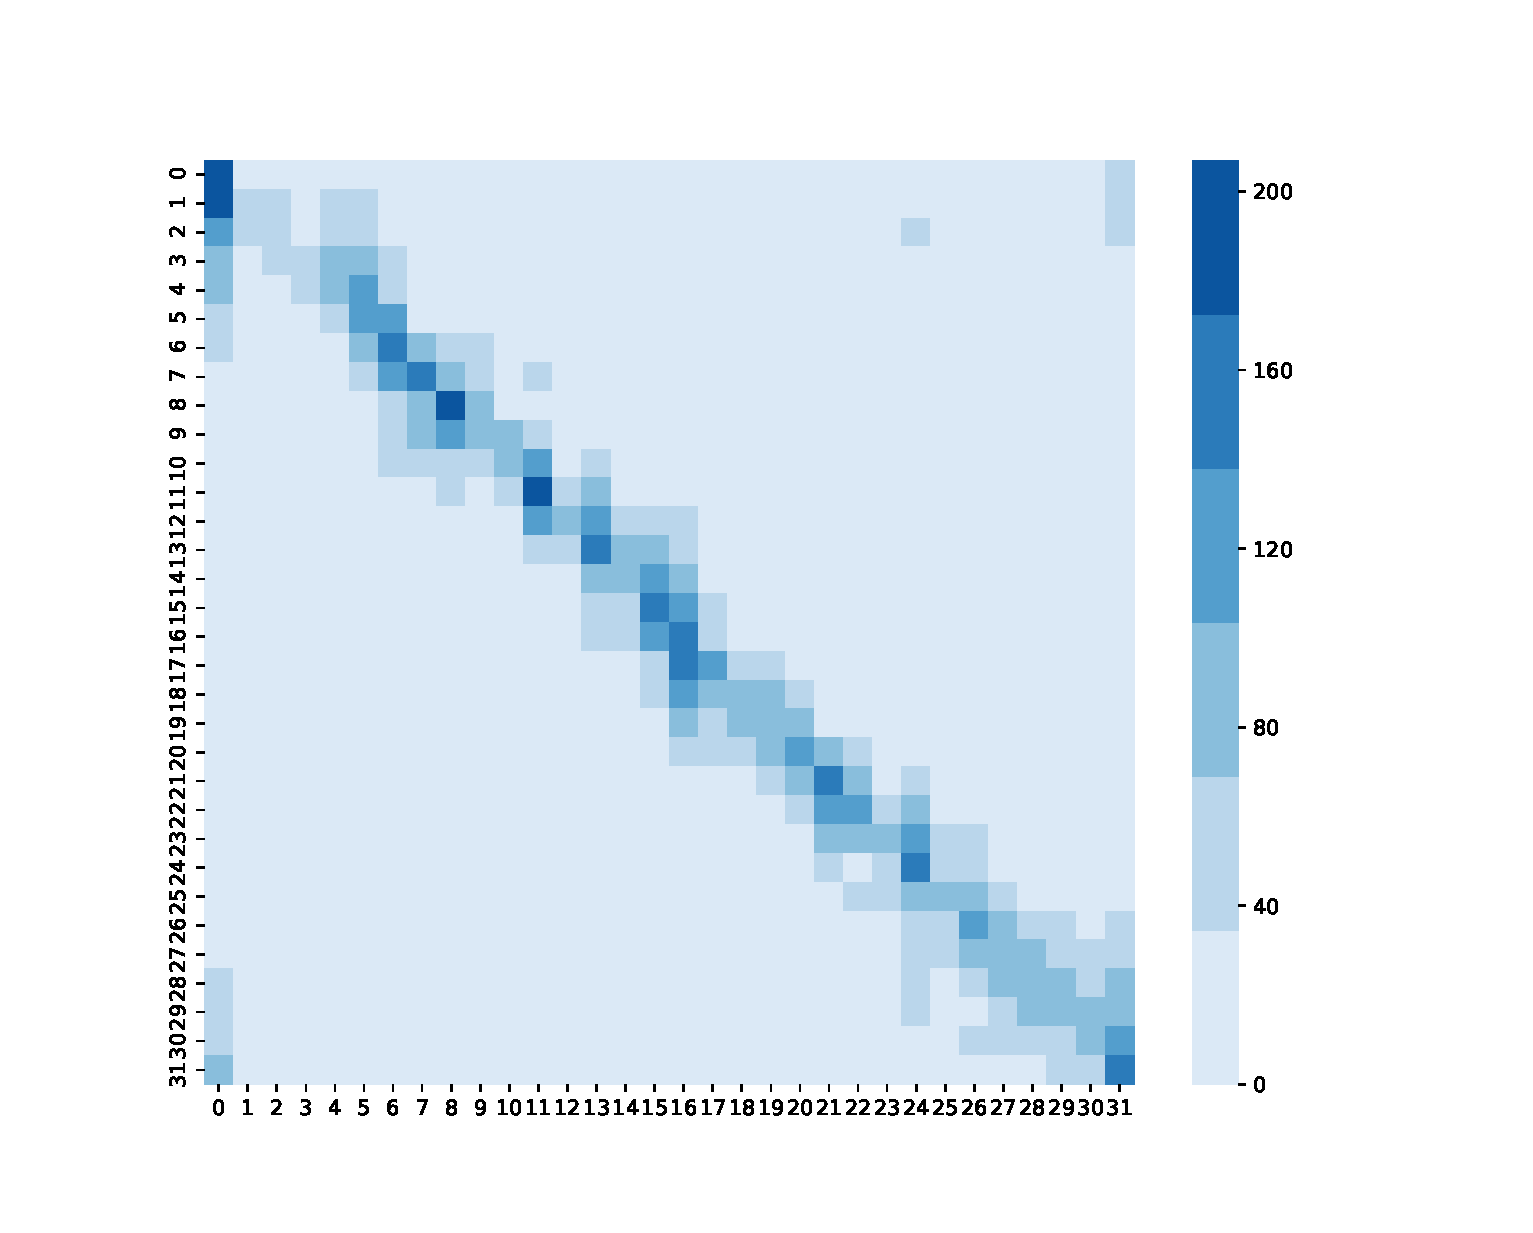
\includegraphics[width=\textwidth,height=\textheight,keepaspectratio]{Figures/confusion-matrix/08-kpt-133049.eps}
    \caption[Confusion matrix obtained after 133049 global steps of model training for blocks of size \(8\times8\)]
    {Confusion matrix obtained after 133049 global steps of model training for blocks of size \(8\times8\)}\label{fig:cm8times8}
\end{figure}

\begin{figure}
    \centering
    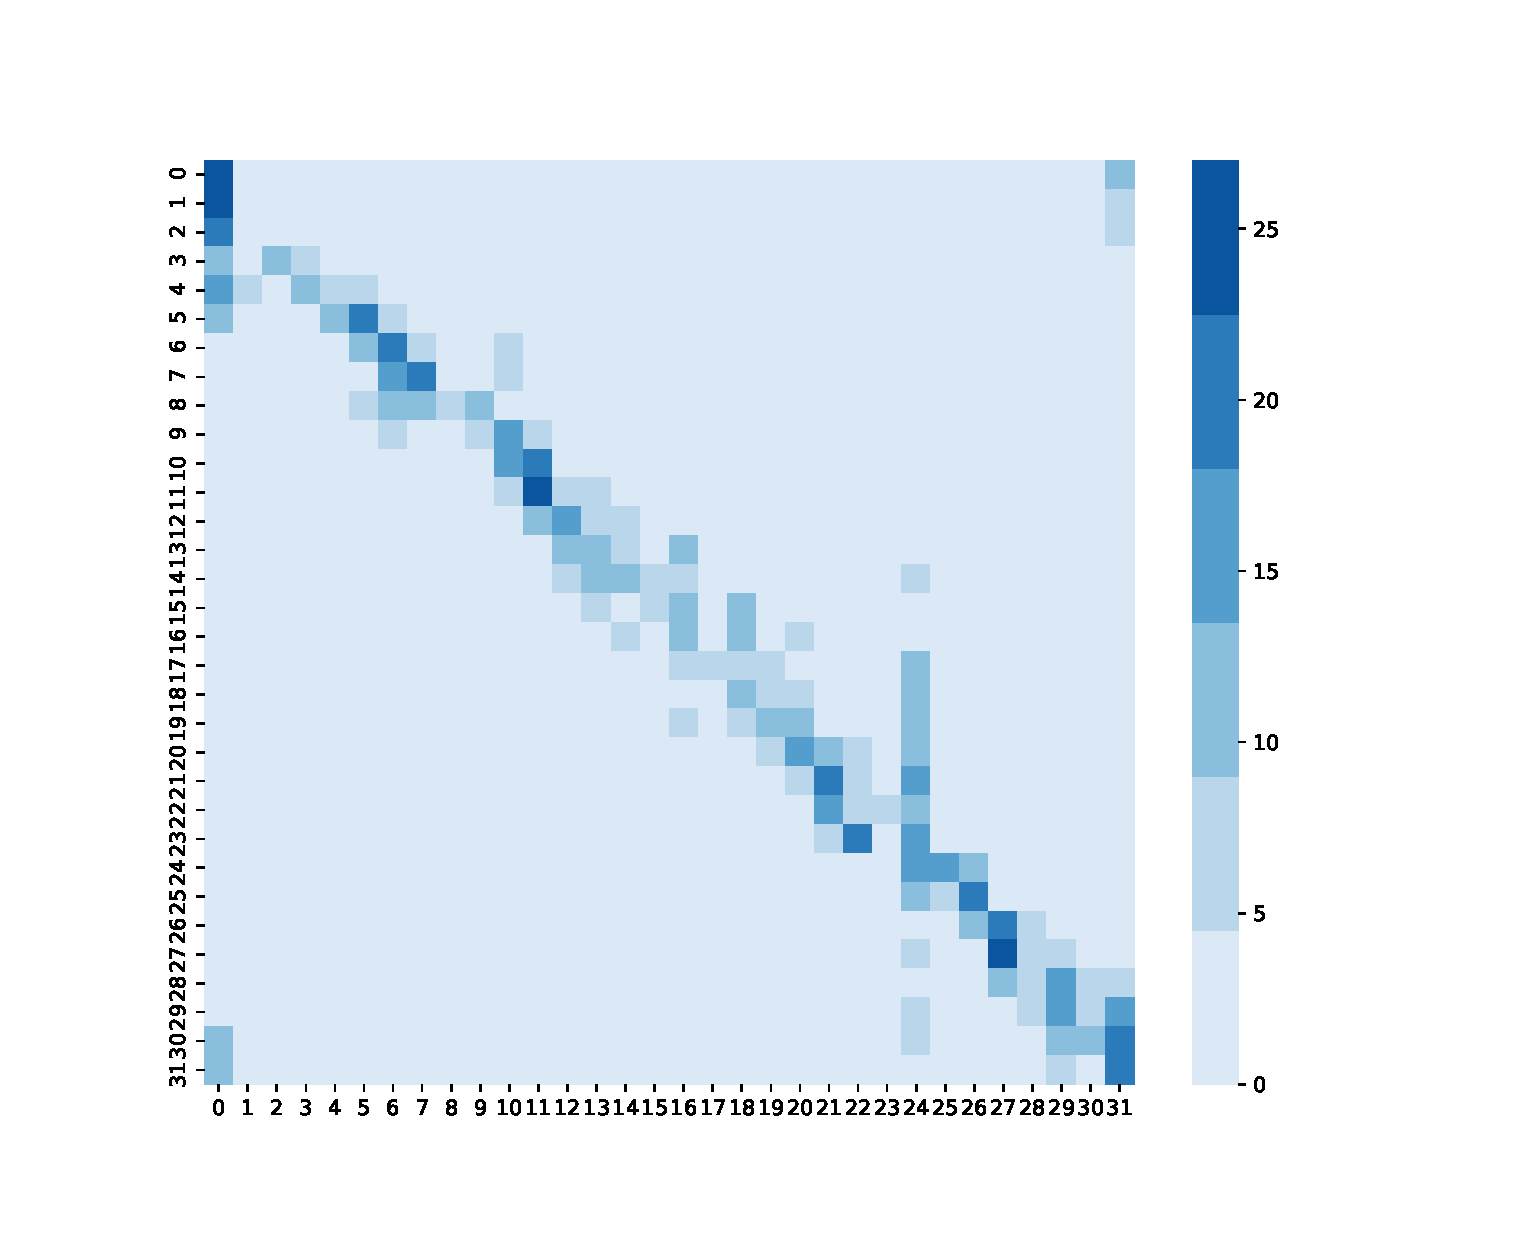
\includegraphics[width=\textwidth,height=\textheight,keepaspectratio]{Figures/confusion-matrix/16-kpt-304857.eps}
    \caption[Top-k precision on testing datasets for each block size]
    {Top-k precision on testing datasets for each block size}\label{fig:cm16times16}
\end{figure}

\section{Evaluate the Learned Models}\label{sec:eval-section}
Two models have been obtained after the training process.
One of the models is is trained from blocks of size \(8\times8\) and 
applied for blocks with the same size.
The other one is trained from blocks of size \(16\times16\), however, 
it is applied for blocks of size \(16\times16\) and size \(32\times32\).
The top-k precision on testing datasets for various 
block sizes is reported in
Table~\ref{tab:valprecision} 
on page~\pageref{tab:valprecision}
(see also Figure~\ref{fig:topkPrecisions}
on page~\pageref{fig:topkPrecisions}
).
Notice that the maximum size for DMM1 wedgelet prediction 
is \(32\times32\), hence there is no need to perform evaluation 
for blocks of size \(64\times64\).
To evaluate performance on blocks of size \(32\times32\),
four resizing methods, i.e., Bilinear Interpolation, 
Nearest Neighbor Interpolation, 
Bicubic Interpolation, and
Area Interpolation,
have been tried.
It turns out the differences among 
the four resizing methods are so trivial
in terms of the prediction accuracies.
Here Bilinear Interpolation
is chosen to be applied in our work.

It can be observed that starting from top-14,
the error rates are all below \(10\% \).
And the model learns well for larger block sizes.
When the models are integrated to the encoder,
if a larger value of \(\mathbf{k}\) is used, 
fewer modes can be excluded which can 
lead to a small time reduction in the encoding process.
In the contrary, if smaller value of \(\mathbf{k}\) is used,
the prediction accuracy may not be high enough
to ensure the encoder performance.
In our work top-15 has been adopted which 
is responsible of balancing
the trade-off between coding performance and 
the time cost in the encoder.



\begin{table}
    \caption{Top-k precision on testing datasets for each block size}
    \bigskip\label{tab:valprecision}
    \centering
    \begin{tabular}{c c c c c}
        \toprule
        \# & Top-k & Size \(8\times8\) & Size \(16\times16\) & Size \(32\times32\) \\
        \midrule
        1 & Top-5 & 0.650     & 0.801  & 0.819 \\
        2 & Top-6  & 0.711    & 0.842  & 0.860 \\
        3 & Top-7  & 0.759    & 0.873  & 0.891 \\
        4 & Top-8  & 0.795    & 0.895  & 0.912 \\
        5 & Top-9  & 0.823    & 0.912  & 0.927 \\
        6 & Top-10  & 0.846   & 0.924   & 0.938 \\
        7 & Top-11  & 0.867   & 0.934   & 0.947 \\
        8 & Top-12  & 0.884   & 0.942   & 0.955 \\
        9 & Top-13  & 0.897   & 0.949   & 0.961 \\
        10 & Top-14  & 0.909  & 0.955   & 0.966 \\
        11 & Top-15  & 0.919  & 0.961   & 0.970 \\
        12 & Top-16  & 0.929  & 0.965   & 0.973 \\
        13 & Top-17  & 0.936  & 0.970   & 0.977 \\
        14 & Top-18  & 0.944  & 0.974   & 0.980 \\
        15 & Top-19  & 0.950  & 0.977   & 0.983 \\
        16 & Top-20  & 0.955  & 0.980   & 0.985 \\
        \bottomrule
    \end{tabular}
\end{table}

\begin{figure}
    \centering
    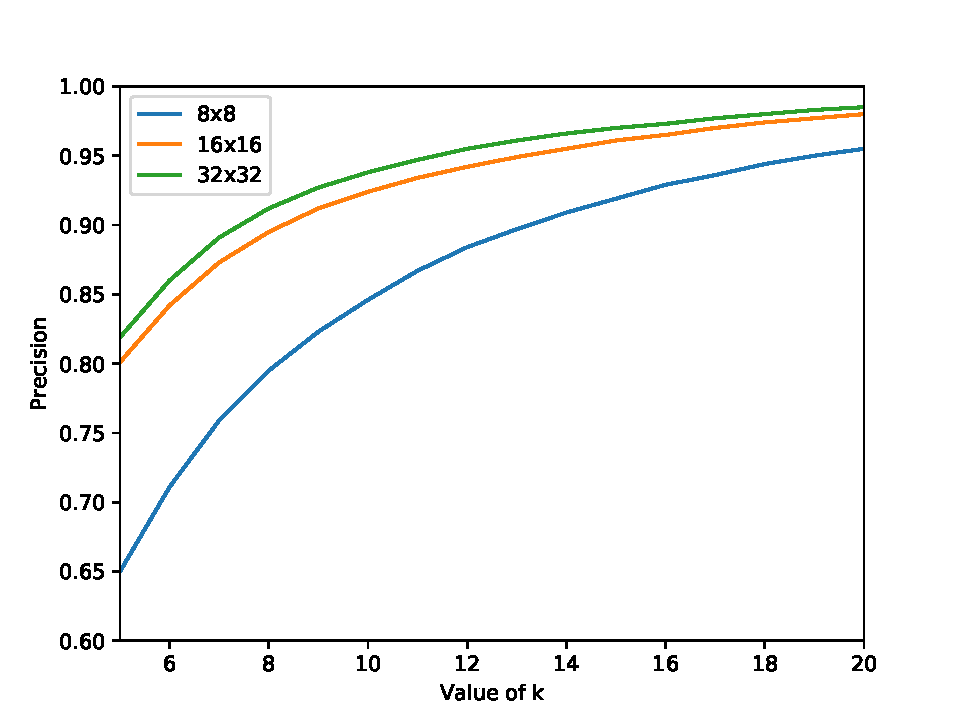
\includegraphics[width=\textwidth,height=\textheight,keepaspectratio]{Figures/topkPrecisions.pdf}
    \caption[Top-k precision on testing datasets for each block size]
    {Top-k precision on testing datasets for each block size}\label{fig:topkPrecisions}
\end{figure}

    \chapter{Evaluate the Learned Deep Model}\label{ch:chapter5} % For referencing the chapter elsewhere, use \ref{Chapter1}
%
%%----------------------------------------------------------------------------------------
%
With the rising popularity of the high definition videos, the new standard
termed High Efficiency Video Coding (HEVC) for compressing videos in a more
efficient way comparing with previous standards, such as H.264/AVC, has
emerged under the efforts from the Joint Collaborative Team on Video
Coding (JCT-VC).
In the meanwhile, five extensions of the HEVC standard, comprising
Format Range Extension (RExt), Scalability Extension (SHVC),
Multi-view Extension (MV-HEVC), 3D Extension (3D-HEVC),
Screen Content Coding Extension (SCC),  have been finalized
from 2014 to 2016 to support fulfill extra requirements in various
scenarios.
%3D Video applications are attracting more interests
%%----------------------------------------------------------------------------------------
%
\section{Video Codhgvingg}\label{sec:vivbndeo-codingasfdgsdfgb}
%Welcome to this \LaTeX{} Thesis Template, a beautiful and easy to use template for writing a thesis using the \LaTeX{} typesetting system.
%
%If you are writing a thesis (or will be in the future) and its subject is technical or mathematical (though it doesn't have to be), then creating it in \LaTeX{} is highly recommended as a way to make sure you can just get down to the essential writing without having to worry over formatting or wasting time arguing with your word processor.
%
%\LaTeX{} is easily able to~\parencite{RN93} professionally typeset documents that run to hundreds or thousands of pages long. With simple mark-up commands, it automatically sets out the table of contents, margins, page headers and footers and keeps the formatting consistent and beautiful. One of its main strengths is the way it can easily typeset mathematics, even \emph{heavy} mathematics. Even if those equations are the most horribly twisted and most difficult mathematical problems that can only be solved on a super-computer, you can at least count on \LaTeX{} to make them look stunning.
%
%%----------------------------------------------------------------------------------------
%
%\section{Welcome and Thanku}\label{sec:welome}
%Welcome to this \LaTeX{} Thesis Template, a beautiful and easy to use template for writing a thesis using the \LaTeX{} typesetting system.
%
%If you are writing a thesis (or will be in the future) and its subject is technical or mathematical (though it doesn't have to be), then creating it in \LaTeX{} is highly recommended as a way to make sure you can just get down to the essential writing without having to worry over formatting or wasting time arguing with your word processor.
%
%\LaTeX{} is easily able to professionally typeset documents that run to hundreds or thousands of pages long. With simple mark-up commands, it automatically sets out the table of contents, margins, page headers and footers and keeps the formatting consistent and beautiful. One of its main strengths is the way it can easily typeset mathematics, even \emph{heavy} mathematics. Even if those equations are the most horribly twisted and most difficult mathematical problems that can only be solved on a super-computer, you can at least count on \LaTeX{} to make them look stunning.
%
%%----------------------------------------------------------------------------------------
%
%\section{Welcome and ThYou}\label{sec:weome}
%Welcome to this \LaTeX{} Thesis Template~\parencite{Reference1}, a beautiful and easy to use template for writing a thesis using the \LaTeX{} typesetting system.
%
%If you are writing a thesis (or will be in the future) and its subject is technical or mathematical (though it doesn't have to be), then creating it in \LaTeX{} is highly recommended as a way to make sure you can just get down to the essential writing without having to worry over formatting or wasting time arguing with your word processor.
%
%\LaTeX{} is easily able to professionally typeset documents that run to hundreds or thousands of pages long. With simple mark-up commands, it automatically sets out the table of contents, margins, page headers and footers and keeps the formatting consistent and beautiful. One of its main strengths is the way it can easily typeset mathematics, even \emph{heavy} mathematics. Even if those equations are the most horribly twisted and most difficult mathematical problems that can only be solved on a super-computer, you can at least count on \LaTeX{} to make them look stunning.
%
%%----------------------------------------------------------------------------------------
%
%\section{Welcome and Thau}\label{sec:welcoe}
%Welcome to this \LaTeX{} Thesis Template, a beautiful and easy to use template for writing a thesis using the \LaTeX{} typesetting system.
%
%If you are
%\begin{table}
%
%    \label{tab:treatments}
%    \centering
%%    \begin{tabular}{l l l}
%%        \toprule
%%        \tabhead{Groups} & \tabhead{Treatment X} & \tabhead{Treatment Y} \\
%%        \midrule
%%        1 & 0.2 & 0.8\\
%%        2 & 0.17 & 0.7\\
%%        3 & 0.24 & 0.75\\
%%        4 & 0.68 & 0.3\\
%%        \bottomrule\\
%%    \end{tabular}
%    \begin{tabular}{c r @{.} l}
%        Pi expression       &
%        \multicolumn{2}{c}{Value} \\
%        \hline
%        $\pi$               & 3&1416  \\
%        $\pi^{\pi}$         & 36&46   \\
%        $(\pi^{\pi})^{\pi}$ & 80662&7 \\
%    \end{tabular}
%    \caption{The effects of treatments X and Y on the four groups studied.}
%\end{table}
%writing a thesis (or will be in the future) and its subject is technical or mathematical (though it doesn't have to be), then creating it in \LaTeX{} is highly recommended as a way to make sure you can just get down to the essential writing without having to worry over formatting or wasting time arguing with your word processor.
%
%\LaTeX{} is easily able to professionally typeset documents that run to hundreds or thousands of pages long. With simple mark-up commands, it automatically sets out the table of contents, margins, page headers and footers and keeps the formatting consistent and beautiful. One of its main strengths is the way it can easily typeset mathematics, even \emph{heavy} mathematics. Even if those equations are the most horribly twisted and most difficult mathematical problems that can only be solved on a super-computer, you can at least count on \LaTeX{} to make them look stunning.
%
%%----------------------------------------------------------------------------------------
%
%\section{Welcome and Tnk You}\label{sec:wlcome}
%Welcome to this \LaTeX{} Thesis Template, a beautiful and easy to use template for writing a thesis using the \LaTeX{} typesetting system.
%
%If you are writing a thesis.
%
%%\begin{verbatim}
%\begin{figure}
%    \centering
%    
\includegraphics{Figures/Electron}
%    %    \decoRule
%    \caption[An Electron]{An electron (artist's impression).}
%    \label{fig:Electron}
%\end{figure}
%%\end{verbatim}
%(or will be in the future) and its subject is technical or mathematical (though it doesn't have to be), then creating it in \LaTeX{} is highly recommended as a way to make sure you can just get down to the essential writing without having to worry over formatting or wasting time arguing with your word processor.
%
%\LaTeX{} is easily able to professionally typeset documents that run to hundreds or thousands of pages long. With simple mark-up commands, it automatically sets out the table of contents, margins, page headers and footers and keeps the formatting consistent and beautiful. One of its main strengths is the way it can easily typeset mathematics, even \emph{heavy} mathematics. Even if those equations are the most horribly twisted and most difficult mathematical problems that can only be solved on a super-computer, you can at least count on \LaTeX{} to make them look stunning.
%
%%----------------------------------------------------------------------------------------
    % !TEX root = ../main.tex
\chapter{Conclusion}\label{ch:chapter6} % For referencing the chapter elsewhere, use \ref{Chapter1}
%
%%----------------------------------------------------------------------------------------
%
With the rising popularity of the high definition videos, the new standard
termed High Efficiency Video Coding (HEVC) for compressing videos in a more
efficient way comparing with previous standards, such as H.264/AVC, has
emerged under the efforts from the Joint Collaborative Team on Video
Coding (JCT-VC).
In the meanwhile, five extensions of the HEVC standard, comprising
Format Range Extension (RExt), Scalability Extension (SHVC),
Multi-view Extension (MV-HEVC), 3D Extension (3D-HEVC),
Screen Content Coding Extension (SCC),  have been finalized
from 2014 to 2016 to support fulfill extra requirements in various
scenarios.
%3D Video applications are attracting more interests
%%----------------------------------------------------------------------------------------
%
%\section{Video Codvbnvnbvcnbvnbing}\label{sec:nvbvnbvnbvnbvvideo-codinasfasdgfg}
%Welcome to this \LaTeX{} Thesis Template, a beautiful and easy to use template for writing a thesis using the \LaTeX{} typesetting system.
%
%If you are writing a thesis (or will be in the future) and its subject is technical or mathematical (though it doesn't have to be), then creating it in \LaTeX{} is highly recommended as a way to make sure you can just get down to the essential writing without having to worry over formatting or wasting time arguing with your word processor.
%
%\LaTeX{} is easily able to~\parencite{RN93} professionally typeset documents that run to hundreds or thousands of pages long. With simple mark-up commands, it automatically sets out the table of contents, margins, page headers and footers and keeps the formatting consistent and beautiful. One of its main strengths is the way it can easily typeset mathematics, even \emph{heavy} mathematics. Even if those equations are the most horribly twisted and most difficult mathematical problems that can only be solved on a super-computer, you can at least count on \LaTeX{} to make them look stunning.
%
%%----------------------------------------------------------------------------------------
%
%\section{Welcome and Thanku}\label{sec:welome}
%Welcome to this \LaTeX{} Thesis Template, a beautiful and easy to use template for writing a thesis using the \LaTeX{} typesetting system.
%
%If you are writing a thesis (or will be in the future) and its subject is technical or mathematical (though it doesn't have to be), then creating it in \LaTeX{} is highly recommended as a way to make sure you can just get down to the essential writing without having to worry over formatting or wasting time arguing with your word processor.
%
%\LaTeX{} is easily able to professionally typeset documents that run to hundreds or thousands of pages long. With simple mark-up commands, it automatically sets out the table of contents, margins, page headers and footers and keeps the formatting consistent and beautiful. One of its main strengths is the way it can easily typeset mathematics, even \emph{heavy} mathematics. Even if those equations are the most horribly twisted and most difficult mathematical problems that can only be solved on a super-computer, you can at least count on \LaTeX{} to make them look stunning.
%
%%----------------------------------------------------------------------------------------
%
%\section{Welcome and ThYou}\label{sec:weome}
%Welcome to this \LaTeX{} Thesis Template~\parencite{Reference1}, a beautiful and easy to use template for writing a thesis using the \LaTeX{} typesetting system.
%
%If you are writing a thesis (or will be in the future) and its subject is technical or mathematical (though it doesn't have to be), then creating it in \LaTeX{} is highly recommended as a way to make sure you can just get down to the essential writing without having to worry over formatting or wasting time arguing with your word processor.
%
%\LaTeX{} is easily able to professionally typeset documents that run to hundreds or thousands of pages long. With simple mark-up commands, it automatically sets out the table of contents, margins, page headers and footers and keeps the formatting consistent and beautiful. One of its main strengths is the way it can easily typeset mathematics, even \emph{heavy} mathematics. Even if those equations are the most horribly twisted and most difficult mathematical problems that can only be solved on a super-computer, you can at least count on \LaTeX{} to make them look stunning.
%
%%----------------------------------------------------------------------------------------
%
%\section{Welcome and Thau}\label{sec:welcoe}
%Welcome to this \LaTeX{} Thesis Template, a beautiful and easy to use template for writing a thesis using the \LaTeX{} typesetting system.
%
%If you are
%\begin{table}
%
%    \label{tab:treatments}
%    \centering
%%    \begin{tabular}{l l l}
%%        \toprule
%%        \tabhead{Groups} & \tabhead{Treatment X} & \tabhead{Treatment Y} \\
%%        \midrule
%%        1 & 0.2 & 0.8\\
%%        2 & 0.17 & 0.7\\
%%        3 & 0.24 & 0.75\\
%%        4 & 0.68 & 0.3\\
%%        \bottomrule\\
%%    \end{tabular}
%    \begin{tabular}{c r @{.} l}
%        Pi expression       &
%        \multicolumn{2}{c}{Value} \\
%        \hline
%        $\pi$               & 3&1416  \\
%        $\pi^{\pi}$         & 36&46   \\
%        $(\pi^{\pi})^{\pi}$ & 80662&7 \\
%    \end{tabular}
%    \caption{The effects of treatments X and Y on the four groups studied.}
%\end{table}
%writing a thesis (or will be in the future) and its subject is technical or mathematical (though it doesn't have to be), then creating it in \LaTeX{} is highly recommended as a way to make sure you can just get down to the essential writing without having to worry over formatting or wasting time arguing with your word processor.
%
%\LaTeX{} is easily able to professionally typeset documents that run to hundreds or thousands of pages long. With simple mark-up commands, it automatically sets out the table of contents, margins, page headers and footers and keeps the formatting consistent and beautiful. One of its main strengths is the way it can easily typeset mathematics, even \emph{heavy} mathematics. Even if those equations are the most horribly twisted and most difficult mathematical problems that can only be solved on a super-computer, you can at least count on \LaTeX{} to make them look stunning.
%
%%----------------------------------------------------------------------------------------
%
%\section{Welcome and Tnk You}\label{sec:wlcome}
%Welcome to this \LaTeX{} Thesis Template, a beautiful and easy to use template for writing a thesis using the \LaTeX{} typesetting system.
%
%If you are writing a thesis.
%
%%\begin{verbatim}
%\begin{figure}
%    \centering
%    
\includegraphics{Figures/Electron}
%    %    \decoRule
%    \caption[An Electron]{An electron (artist's impression).}
%    \label{fig:Electron}
%\end{figure}
%%\end{verbatim}
%(or will be in the future) and its subject is technical or mathematical (though it doesn't have to be), then creating it in \LaTeX{} is highly recommended as a way to make sure you can just get down to the essential writing without having to worry over formatting or wasting time arguing with your word processor.
%
%\LaTeX{} is easily able to professionally typeset documents that run to hundreds or thousands of pages long. With simple mark-up commands, it automatically sets out the table of contents, margins, page headers and footers and keeps the formatting consistent and beautiful. One of its main strengths is the way it can easily typeset mathematics, even \emph{heavy} mathematics. Even if those equations are the most horribly twisted and most difficult mathematical problems that can only be solved on a super-computer, you can at least count on \LaTeX{} to make them look stunning.
%
%%----------------------------------------------------------------------------------------
    % % !TEX root = ../main.tex
\chapter{Conclusion}\label{ch:chapter7} % For referencing the chapter elsewhere, use \ref{Chapter1}
%
%%----------------------------------------------------------------------------------------
%
With the rising popularity of the high definition videos, the new standard
termed High Efficiency Video Coding (HEVC) for compressing videos in a more
efficient way comparing with previous standards, such as H.264/AVC, has
emerged under the efforts from the Joint Collaborative Team on Video
Coding (JCT-VC).
In the meanwhile, five extensions of the HEVC standard, comprising
Format Range Extension (RExt), Scalability Extension (SHVC),
Multi-view Extension (MV-HEVC), 3D Extension (3D-HEVC),
Screen Content Coding Extension (SCC),  have been finalized
from 2014 to 2016 to support fulfill extra requirements in various
scenarios.
%3D Video applications are attracting more interests
%%----------------------------------------------------------------------------------------
%
%\section{Video Codvbnvnbvcnbvnbing}\label{sec:nvbvnbvnbvnbvvideo-codinasfasdgfg}
%Welcome to this \LaTeX{} Thesis Template, a beautiful and easy to use template for writing a thesis using the \LaTeX{} typesetting system.
%
%If you are writing a thesis (or will be in the future) and its subject is technical or mathematical (though it doesn't have to be), then creating it in \LaTeX{} is highly recommended as a way to make sure you can just get down to the essential writing without having to worry over formatting or wasting time arguing with your word processor.
%
%\LaTeX{} is easily able to~\parencite{RN93} professionally typeset documents that run to hundreds or thousands of pages long. With simple mark-up commands, it automatically sets out the table of contents, margins, page headers and footers and keeps the formatting consistent and beautiful. One of its main strengths is the way it can easily typeset mathematics, even \emph{heavy} mathematics. Even if those equations are the most horribly twisted and most difficult mathematical problems that can only be solved on a super-computer, you can at least count on \LaTeX{} to make them look stunning.
%
%%----------------------------------------------------------------------------------------
%
%\section{Welcome and Thanku}\label{sec:welome}
%Welcome to this \LaTeX{} Thesis Template, a beautiful and easy to use template for writing a thesis using the \LaTeX{} typesetting system.
%
%If you are writing a thesis (or will be in the future) and its subject is technical or mathematical (though it doesn't have to be), then creating it in \LaTeX{} is highly recommended as a way to make sure you can just get down to the essential writing without having to worry over formatting or wasting time arguing with your word processor.
%
%\LaTeX{} is easily able to professionally typeset documents that run to hundreds or thousands of pages long. With simple mark-up commands, it automatically sets out the table of contents, margins, page headers and footers and keeps the formatting consistent and beautiful. One of its main strengths is the way it can easily typeset mathematics, even \emph{heavy} mathematics. Even if those equations are the most horribly twisted and most difficult mathematical problems that can only be solved on a super-computer, you can at least count on \LaTeX{} to make them look stunning.
%
%%----------------------------------------------------------------------------------------
%
%\section{Welcome and ThYou}\label{sec:weome}
%Welcome to this \LaTeX{} Thesis Template~\parencite{Reference1}, a beautiful and easy to use template for writing a thesis using the \LaTeX{} typesetting system.
%
%If you are writing a thesis (or will be in the future) and its subject is technical or mathematical (though it doesn't have to be), then creating it in \LaTeX{} is highly recommended as a way to make sure you can just get down to the essential writing without having to worry over formatting or wasting time arguing with your word processor.
%
%\LaTeX{} is easily able to professionally typeset documents that run to hundreds or thousands of pages long. With simple mark-up commands, it automatically sets out the table of contents, margins, page headers and footers and keeps the formatting consistent and beautiful. One of its main strengths is the way it can easily typeset mathematics, even \emph{heavy} mathematics. Even if those equations are the most horribly twisted and most difficult mathematical problems that can only be solved on a super-computer, you can at least count on \LaTeX{} to make them look stunning.
%
%%----------------------------------------------------------------------------------------
%
%\section{Welcome and Thau}\label{sec:welcoe}
%Welcome to this \LaTeX{} Thesis Template, a beautiful and easy to use template for writing a thesis using the \LaTeX{} typesetting system.
%
%If you are
%\begin{table}
%
%    \label{tab:treatments}
%    \centering
%%    \begin{tabular}{l l l}
%%        \toprule
%%        \tabhead{Groups} & \tabhead{Treatment X} & \tabhead{Treatment Y} \\
%%        \midrule
%%        1 & 0.2 & 0.8\\
%%        2 & 0.17 & 0.7\\
%%        3 & 0.24 & 0.75\\
%%        4 & 0.68 & 0.3\\
%%        \bottomrule\\
%%    \end{tabular}
%    \begin{tabular}{c r @{.} l}
%        Pi expression       &
%        \multicolumn{2}{c}{Value} \\
%        \hline
%        $\pi$               & 3&1416  \\
%        $\pi^{\pi}$         & 36&46   \\
%        $(\pi^{\pi})^{\pi}$ & 80662&7 \\
%    \end{tabular}
%    \caption{The effects of treatments X and Y on the four groups studied.}
%\end{table}
%writing a thesis (or will be in the future) and its subject is technical or mathematical (though it doesn't have to be), then creating it in \LaTeX{} is highly recommended as a way to make sure you can just get down to the essential writing without having to worry over formatting or wasting time arguing with your word processor.
%
%\LaTeX{} is easily able to professionally typeset documents that run to hundreds or thousands of pages long. With simple mark-up commands, it automatically sets out the table of contents, margins, page headers and footers and keeps the formatting consistent and beautiful. One of its main strengths is the way it can easily typeset mathematics, even \emph{heavy} mathematics. Even if those equations are the most horribly twisted and most difficult mathematical problems that can only be solved on a super-computer, you can at least count on \LaTeX{} to make them look stunning.
%
%%----------------------------------------------------------------------------------------
%
%\section{Welcome and Tnk You}\label{sec:wlcome}
%Welcome to this \LaTeX{} Thesis Template, a beautiful and easy to use template for writing a thesis using the \LaTeX{} typesetting system.
%
%If you are writing a thesis.
%
%%\begin{verbatim}
%\begin{figure}
%    \centering
%    
\includegraphics{Figures/Electron}
%    %    \decoRule
%    \caption[An Electron]{An electron (artist's impression).}
%    \label{fig:Electron}
%\end{figure}
%%\end{verbatim}
%(or will be in the future) and its subject is technical or mathematical (though it doesn't have to be), then creating it in \LaTeX{} is highly recommended as a way to make sure you can just get down to the essential writing without having to worry over formatting or wasting time arguing with your word processor.
%
%\LaTeX{} is easily able to professionally typeset documents that run to hundreds or thousands of pages long. With simple mark-up commands, it automatically sets out the table of contents, margins, page headers and footers and keeps the formatting consistent and beautiful. One of its main strengths is the way it can easily typeset mathematics, even \emph{heavy} mathematics. Even if those equations are the most horribly twisted and most difficult mathematical problems that can only be solved on a super-computer, you can at least count on \LaTeX{} to make them look stunning.
%
%%----------------------------------------------------------------------------------------
%    \appendix
    % \chapter{Algorithm for Data Collection}\label{ch:app-algo-data-collection}
%    \chapter{Visualizations of Raw Data}\label{ch:app-visu}
    \printbibliography[heading=bibintoc]
\end{document}
